%%%%%%%%%%%%%%%%%%%%%%%%%%%%%%%%%%%%%%%%%%%%%%%%%%%%%%%%%%%%%%%%%%%%%%%%%%%%%%%%
%2345678901234567890123456789012345678901234567890123456789012345678901234567890
%        1         2         3         4         5         6         7         8

\documentclass[journal,transmag]{IEEEtran}% Comment this line out if you need a4paper

%\documentclass[a4paper, 10pt, conference]{ieeeconf}      % Use this line for a4 paper

\IEEEoverridecommandlockouts                              % This command is only needed if 
                                                          % you want to use the \thanks command

%\overrideIEEEmargins                                      % Needed to meet printer requirements.

% See the \addtolength command later in the file to balance the column lengths
% on the last page of the document

% The following packages can be found on http:\\www.ctan.org
%\usepackage{graphics} % for pdf, bitmapped graphics files
%\usepackage{epsfig} % for postscript graphics files
%\usepackage{mathptmx} % assumes new font selection scheme installed
%\usepackage{times} % assumes new font selection scheme installed
%\usepackage{amsmath} % assumes amsmath package installed
%\usepackage{amssymb}  % assumes amsmath package installed



\usepackage{amsmath,amssymb}

\usepackage{tikz,hyperref,graphicx,units,subfig}
\usepackage{subfig}
\usepackage{benktools}
\usepackage{caption}
\renewcommand{\captionfont}{\footnotesize}
\usepackage{sidecap,wrapfig}
\usepackage[ruled,vlined]{algorithm2e}
\DeclareMathOperator*{\argmin}{arg\,min}
\DeclareMathOperator*{\argmax}{arg\,max}
\newcommand{\abs}[1]{\lvert#1\rvert} 
\newcommand{\norm}[1]{\lVert#1\rVert}
%\newcommand{\suchthat}{\mid}
\newcommand{\suchthat}{\ \big|\ }
\newcommand{\bd}{\mathbf{d}}
\newcommand{\bn}{\mathbf{n}}
\newcommand{\bp}{\mathbf{p}}
\newcommand{\bw}{\mathbf{w}}
\newcommand{\bt}{\mathbf{t}}
\newcommand{\by}{\mathbf{y}}
\newcommand{\bx}{\mathbf{x}}
\newcommand{\bz}{\mathbf{z}}
\newcommand{\bbf}{\mathbf{f}}
\newcommand{\bzero}{\mathbf{0}}
\newcommand{\bG}{\mathbf{G}}
\newcommand{\bA}{\mathbf{A}}
\newcommand{\bW}{\mathbf{W}}
\newcommand{\bX}{\mathbf{X}}
\newcommand{\mX}{\mathcal{X}}
\newcommand{\mD}{\mathcal{D}}
\newcommand{\mN}{\mathcal{N}}
\newcommand{\mW}{\mathcal{W}}
\newcommand{\mF}{\mathcal{F}}
\newcommand{\bZ}{\mathbf{Z}}

\newcommand{\bfc}{W}
\newcommand{\Qinf}{Q_{\infty}}
\newcommand{\st}[1]{_\text{#1}}
\newcommand{\rres}{r\st{res}}
\newcommand{\pos}[1]{(#1)^+}
\newcommand{\depth}{\operatorname{depth}}
\newcommand{\dist}{\operatorname{dist}}
\newcommand{\convhull}{\operatorname{ConvexHull}}
\newcommand{\minksum}{\operatorname{MinkowskiSum}}

\title{\LARGE \bf
Efficient Planar Sample-Based Grasp Planning with Uncertainty Using Budgeted Multi-Armed Bandit Models for  [v3 Jan 5, 2015 ] }


\author{Michael Laskey$^1$,Jeff Mahler$^1$, Zoe McCarthy$^1$,  Florian T. Pokorny$^3$, Sachin Patil$^1$,\\ Jur Van Den Berg$^4$,  Danica Kragic$^3$, Pieter Abbeel$^1$, Ken Goldberg$^2$% <-this % stops a space
\thanks{$^1$Department of Electrical Engineering and Computer Sciences; {\small \{mdlaskey, zmccarthy, jmahler, sachinpatil, pabbeel\}@berkeley.edu}}%
\thanks{$^2$Department of Industrial Engineering and Operations Research and Department of Electrical Engineering and Computer Sciences; {\small goldberg@berkeley.edu}}%
\thanks{$^{1-2}$ University of California, Berkeley;  Berkeley, CA 94720, USA}%
\thanks{$^3$Computer Vision and Active Perception Lab, Centre for Autonomous Systems, School of Computer Science and Communication, KTH Royal Institute of Technology, Stockholm, Sweden {\small \{fpokorny, dani\}@kth.se}}%
\thanks{$^4$Google; Amphitheatre Parkway, Mountain View, CA 94043, USA {\small jurvandenberg@gmail.com}}%
} 

\newtheorem{theorem}{Theorem}

\begin{document}



\maketitle
\thispagestyle{empty}
\pagestyle{empty}


%%%%%%%%%%%%%%%%%%%%%%%%%%%%%%%%%%%%%%%%%%%%%%%%%%%%%%%%%%%%%%%%%%%%%%%%%%%%%%%%

\begin{abstract}
\textit{Abstract---}\todo{Not sure if we need to change the authors list or not}Sampling perturbations in shape, state, and control can facilitate grasp planning in the presence of uncertainty arising from noise, occlusions, and surface properties such as transparency and specularities.  Monte-Carlo sampling is computationally demanding, even for planar models. We consider an alternative based on the multi-armed bandit (MAB) model for making sequential decisions, which can apply to a variety of uncertainty models.  We formulate grasp planning as a ``budgeted multi-armed bandit model" (BMAB) with finite stopping time to minimize ``simple regret", the difference between the expected quality of the best grasp and the expected quality of the grasp evaluated at the stopping time.  To evaluate MAB-based sampling, we compare it with Monte-Carlo sampling for grasping an uncertain planar object with shape uncertainty defined by a Gaussian process implicit surface (GPIS), but the method is also applicable to other models of uncertainty.  We derive distributions on contact points, surface normal, and center of mass under shape uncertainty and use these to formulate the associated MAB model, finding that it computes grasps of similar quality to Monte-Carlo sampling and can reduce computation time by an order of magnitude.  This suggests a number of new research questions about how MAB can be applied to other models of uncertainty and how different MAB solution techniques can be applied to further reduce computation.
\end{abstract}

\begin{abstract}
\textit{Note to Practitioners---}Planning for a grasp in an unknown environment can be difficult due to uncertainties. For example, a given object may have transparency which makes modern kinect-like sensor unable to accurately determine shape or an object may have a built up of mildew or dust, which makes the friction coefficient unknown. To handle all the uncertainties and plan for grasps using a grasp metric, one must perform monte-carlo integration and exhaustively evaluate samples. We show that by using simple algorithms from the Multi-Armed bandit literature, you can intelligently decided which grasp to sample from next and quickly determine the best grasp in a given set of proposed grasps, thus helping to alleviate the computational burden that is associated to incorporating uncertainty. 
\end{abstract}
%%%%%%%%%%%%%%%%%%%%%%%%%%%%%%%%%%%%%%%%%%%%%%%%%%%%%%%%%%%%%%%%%%%%%%%%%%%%%%%%

\section{Introduction}


%\vspace{10pt}
%\todo{Get High res GPIS visualizations, Incorporate next round of feedback}

Consider a robot processing orders in a warehouse , where it frequently encounter new consumer products and need to process them quickly.
The robot may need to rapidly plan grasps for these objects without prior knowledge of their shape, pose and material properties like friction coefficient or center of mass. 
Furthermore, the robot may not be able to measure these quantities exactly due to sensor noise and missing data resulting from occlusions and object properties such as transparency or reflective surfaces .

\begin{figure}%
    \centering
     \subfloat{{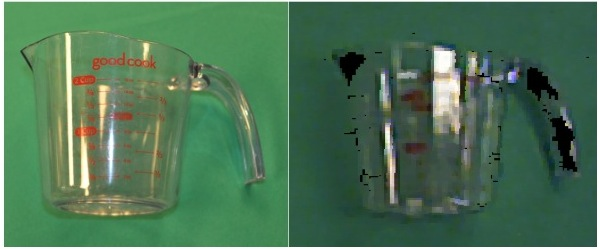
\includegraphics[width=8cm]{figures/cup.jpg} }}%
    
       \qquad
  
     \subfloat{{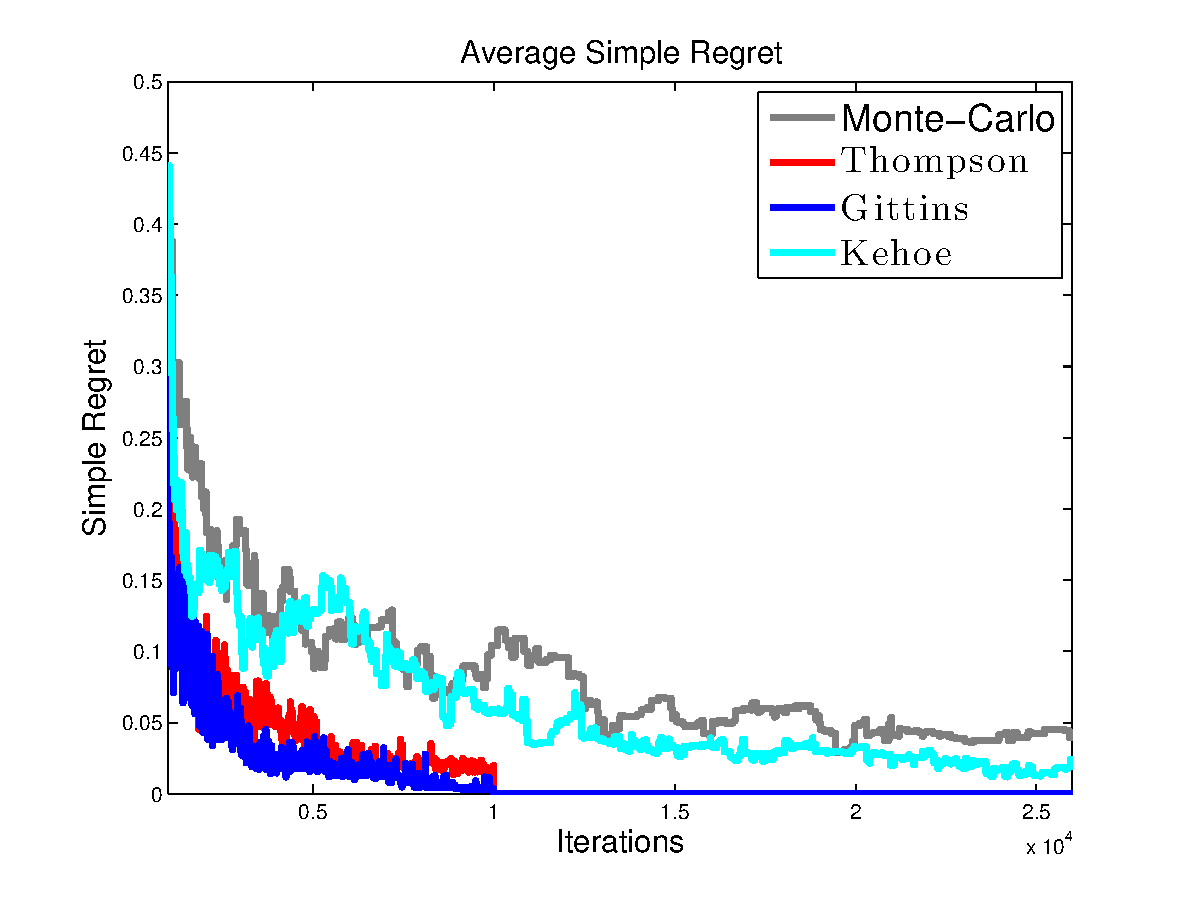
\includegraphics[width=8cm]{matlab_figures/teaser.eps} }}%
   
    \caption{\todo{New teaser photo, not sure if we should have some sort of real object or not}(Top Left) Image of a common household measuring cup. (Top Right) Image from a PR2 Primesense camera that reflects the uncertainty that can be induced in objects from transparency. (Bottom) Comparision of Multi-Armed Bandit Techniques (Bayes UCB, Thompson, Gittins) vs. Monte-Carlo sampling to determine the best grasp in a set of 1000 grasps. As you can see the bandit techniques converge in simple regret Eq. \ref{eq:simple_regret} a magnitude faster than the traditional approach of Monte-Carlo sampling to determine the highest quality grasp.  }%
    \label{fig:rot_shapes}%
\end{figure}

Grasp quality metrics have been developed to determine if a grasp will be successful or not prior to actually executing the grasp and how much force it needs to exert to resist an opposing force, however the ones that we consider evaluate a grasp assuming all the parameters are known \cite{ferrari1992}.
Recent work \cite{kehoe2012estimating,mahler2015gp} motivated using knowledge of uncertainty to select grasps, but most methods for evaluating grasp quality in the presence of uncertainty use Monte Carlo sampling over the possible values of the uncertain quantity \cite{kim2012physically, weisz2012pose}.

To select a grasp with high quality this evaluation is usually performed for a large set of perturbations in state, shape, and material properties, which can be very time-consuming.
However, when evaluating a set of grasps we may be able to determine the difference of quality between proposed grasps with only a few samples and adaptively choose what grasp to evaluate next. We can concentrate grasp quality evaluation on the grasps that are most likely to have the highest quality based on the evaluation done so far.


The multi-armed bandit (MAB) model for sequential decision making problems \cite{barto1998reinforcement, lai1985asymptotically, robbins1952some} provides a way to reason about selecting the next option to evaluate.
The goal in a MAB model is to make a sequence of decisions over a set of possible options, or ``arms", such that a measure of expected reward is maximized.
Solutions to the MAB model are particularly useful in applications where it is too expensive to fully evaluate a set of options; for example, in optimal design of clinical trials~\cite{simon1989optimal}, market pricing~\cite{rothschild1974two}, and choosing strategies for games~\cite{st2012online}.
The budgeted multi-armed bandit model \cite{madani2004budgeted} is a specialization of the MAB model where at a given "stopping time" the agent must choose the arm that currently has the highest expected reward based on its observations. 
The objective is to maximize the expected reward of the decision made at the stopping time, or equivalently to minimize ``simple regret", which is the difference between the true expected reward of an optimal arm and the true expected reward of the arm pulled at the stopping time.

Our main contribution is formulating the problem of planning grasps according to some quality metric in the presence of uncertainty as a budgeted multi-armed bandit model.
We use this formulation to rank a set of potential grasps by the probability of force closure \cite{christopoulos2007handling, kehoe2012toward} under uncertainty in pose, shape, motion and friction coefficient. 
We choose the model of shape uncertainty to be a Gaussian process implicit surface (GPIS), a Bayesian representation of shape uncertainty that has been used in various robotic applications~\cite{dragiev2011, hollinger2013}.  Uncertainty in pose is represented as a normal distributions around the orientation and translation of the object. Uncertainity in motion is represented as a normal distribution around the end point of a planned gripper trajectory and uncertainty in friction coefficient is a normal distribution around an expected friction coefficient.  Our approach of treating grasp selection as a BMAB requires only the ability to sample from a given representation of uncertainty and is not restricted to aforementioned representations. 

We also show how to estimate distributions on the contact points and surface normals and center of mass using GPIS representation for shape uncertainty. Our experiments demonstrate that using the MAB sampling method improves the time to find the best grasp in a set of 1000 grasps by 5x over the baseline Monte-Carlo approach. 
\todo{Going to get a table with results}

\section{Related Work}

Past work on grasping under uncertainty has considered shape uncertainty \cite{goldberg1990bayesian, stulp2011learning}, uncertainty in contact locations with an object \cite{zheng2005}, uncertainty in object pose \cite{christopoulos2007handling, weisz2012pose, kim2012physically}.
The effect of uncertainty in object geometry on grasp selection has been studied for spline representations of objects~\cite{christopoulos2007handling}, extruded polygonal mesh models~\cite{kehoe2012estimating, kehoe2012toward}, and point clouds~\cite{hsiao2011bayesian}.

One method of evaluating the expected grasp quality under uncertainty is to rank a set of random grasps on an object using  samples on shapes, pose or parameters to evaluate a quality measure~\cite{christopoulos2007handling, kehoe2012estimating, kehoe2012toward}.
Monte-Carlo sampling involves drawing random samples from a distribution to approximate an expected value\cite{caflisch1998monte}, which can be slow when the distribution is high-dimensional, such as for distributions on possible shapes.

To address this, Kehoe et al.~\cite{kehoe2012estimating} demonstrated a procedure for finding a minimum bound on expected grasp quality given shape uncertainty, which reduced the number of samples needed in Monte-Carlo sampling to choose the highest quality grasps. However, the proposed adaptive sampling approach pruned grasps using only the sample mean and did not utilize any estimates of how accurate the current sample mean is, which in practice could lead to good grasps being thrown away.
Laaksonen et al.~\cite{laaksonen2012probabilistic} used Markov Chain Monte-Carlo (MCMC) sampling to estimate grasp quality and object pose  under shape and pose uncertainty when the robot is able to obtain new information via tactile sensor.
MCMC provides a Bayesian framework for inference with a hidden state, but it can be slow to converge to the correct distribution due to burn in and mixing conditions~\cite{andrieu2003introduction}.

We chose to study our MAB sampling method on distributions for friction coefficient, pose, motion and shape. For shape uncertainty we decided to use a Gaussian process implicit surface representation. Our decision to use this uncertainty model is based on GPIS's ability to combine different modes of noise observations such as tactile, laser and visual~\cite{rasmussen2006, williams2007, dragiev2011} and its recent use in modeling uncertainty for a number of robotic applications.
Hollinger et al. used GPIS as a model of uncertainty to perform active sensing on the hulls in underwater boats \cite{hollinger2013}.
Dragiev et al. showed how GPIS can enable a grasp controller on the continuous signed distance function \cite{dragiev2011}.
Mahler et al. used the GPIS representation to find locally optimal anti-podal grasps by framing grasp planning as an optimization problem \cite{mahler2015gp}.  However, this relied on an approximation to grasp quality without guarantees on accuracy. We propose an adaptive sampling approach known as the Multi-Armed Bandit Model. This paper is a substantially revised and expanded version on \cite{laskey} and \cite{mahler2015gp}.




\section{Preliminaries and Problem Definition}
Before we present the problem definition, we introduce a way to evaluate the quality of a grasp and our grasping model, the line of action. We also introduce a graphical model to represent the distributions on friction coefficient, motion, pose and shape. 

\subsection{Grasp Metric}
Ferrari and Canny \cite{ferrari1992} demonstrated a method to rank grasps by considering points of contact with an object and the object surface normals at those contacts. The magnitude of the metric allows one to rank grasps by their ability to resist external wrenches (forces and torques) applied to the grasped object. The Ferrari-Canny metric has wide spread use in grasp packages like GraspIT\cite{miller2004graspit}, OpenGrasp\cite{73} and Simox \cite{vahrenkamp2010simo}, which motivates studying its effect with uncertainties. 

Let Q be the $L^1$ version of the metric depends on the contact points $\textbf{c}_1,...,\textbf{c}_m \in \mathcal{R}^2$, surface normals $\textbf{n}_1,...,\textbf{n}_m \in \mathcal{R}^2$, center of mass $\textbf{z}$ and friction coefficient $\mu$. The metric is evaluated by constructing a convex hull around the wrenches made up of those parameters and finding the radius of the largest unit ball centered at the origin in wrench space. If the convex hull  encloses the origin then the grasp is in ``force-closure,'' meaning the grasp can resist any external wrenches if enough force is used. A grasp can be parameterized by the following tuple $g = ( \textbf{c}_1,...,\textbf{c}_m,\textbf{n}_1,...,\textbf{n}_m,\mu, \textbf{z} )$\cite{pokorny2013classical}.

In this work we use the probability of achieving force closure, or $P(Q>0)$, \cite{christopoulos2007handling}\cite{kehoe2012toward}, to rank grasps . $P(Q>0)$ may be computed by sampling from distributions on pose (rotation and translation of the object), shape and material properties (friction coefficient) and averaging the qualities that are computed.

\subsection{Line of action}
In an uncertain environment, a grasp planner may not know the true grasp parameters or $g$ exactly due to sensing imprecision. Thus we propose to work with the trajectory of the gripper when analyzing grasps. Similar to the work of \cite{christopoulos2007handling}, we assume that each gripper finger approaches along a \textit{line of action}, a 1D curve $\gamma(t)$ with endpoints $a$ and $b$ as seen in Fig. \ref{fig:line_of_action}.
A gripper finger starts at point $a$ and moves towards $b$, we assume $a$ is far enough away to be collision free of the object.
Each gripper contact is defined by a line of action, so we assume the following tuple is provided $\Gamma = ( \gamma_1(\cdot),...,\gamma_m(\cdot) )$, which designates a proposed \textit{grasp plan}.

\begin{figure}[ht!]
\centering
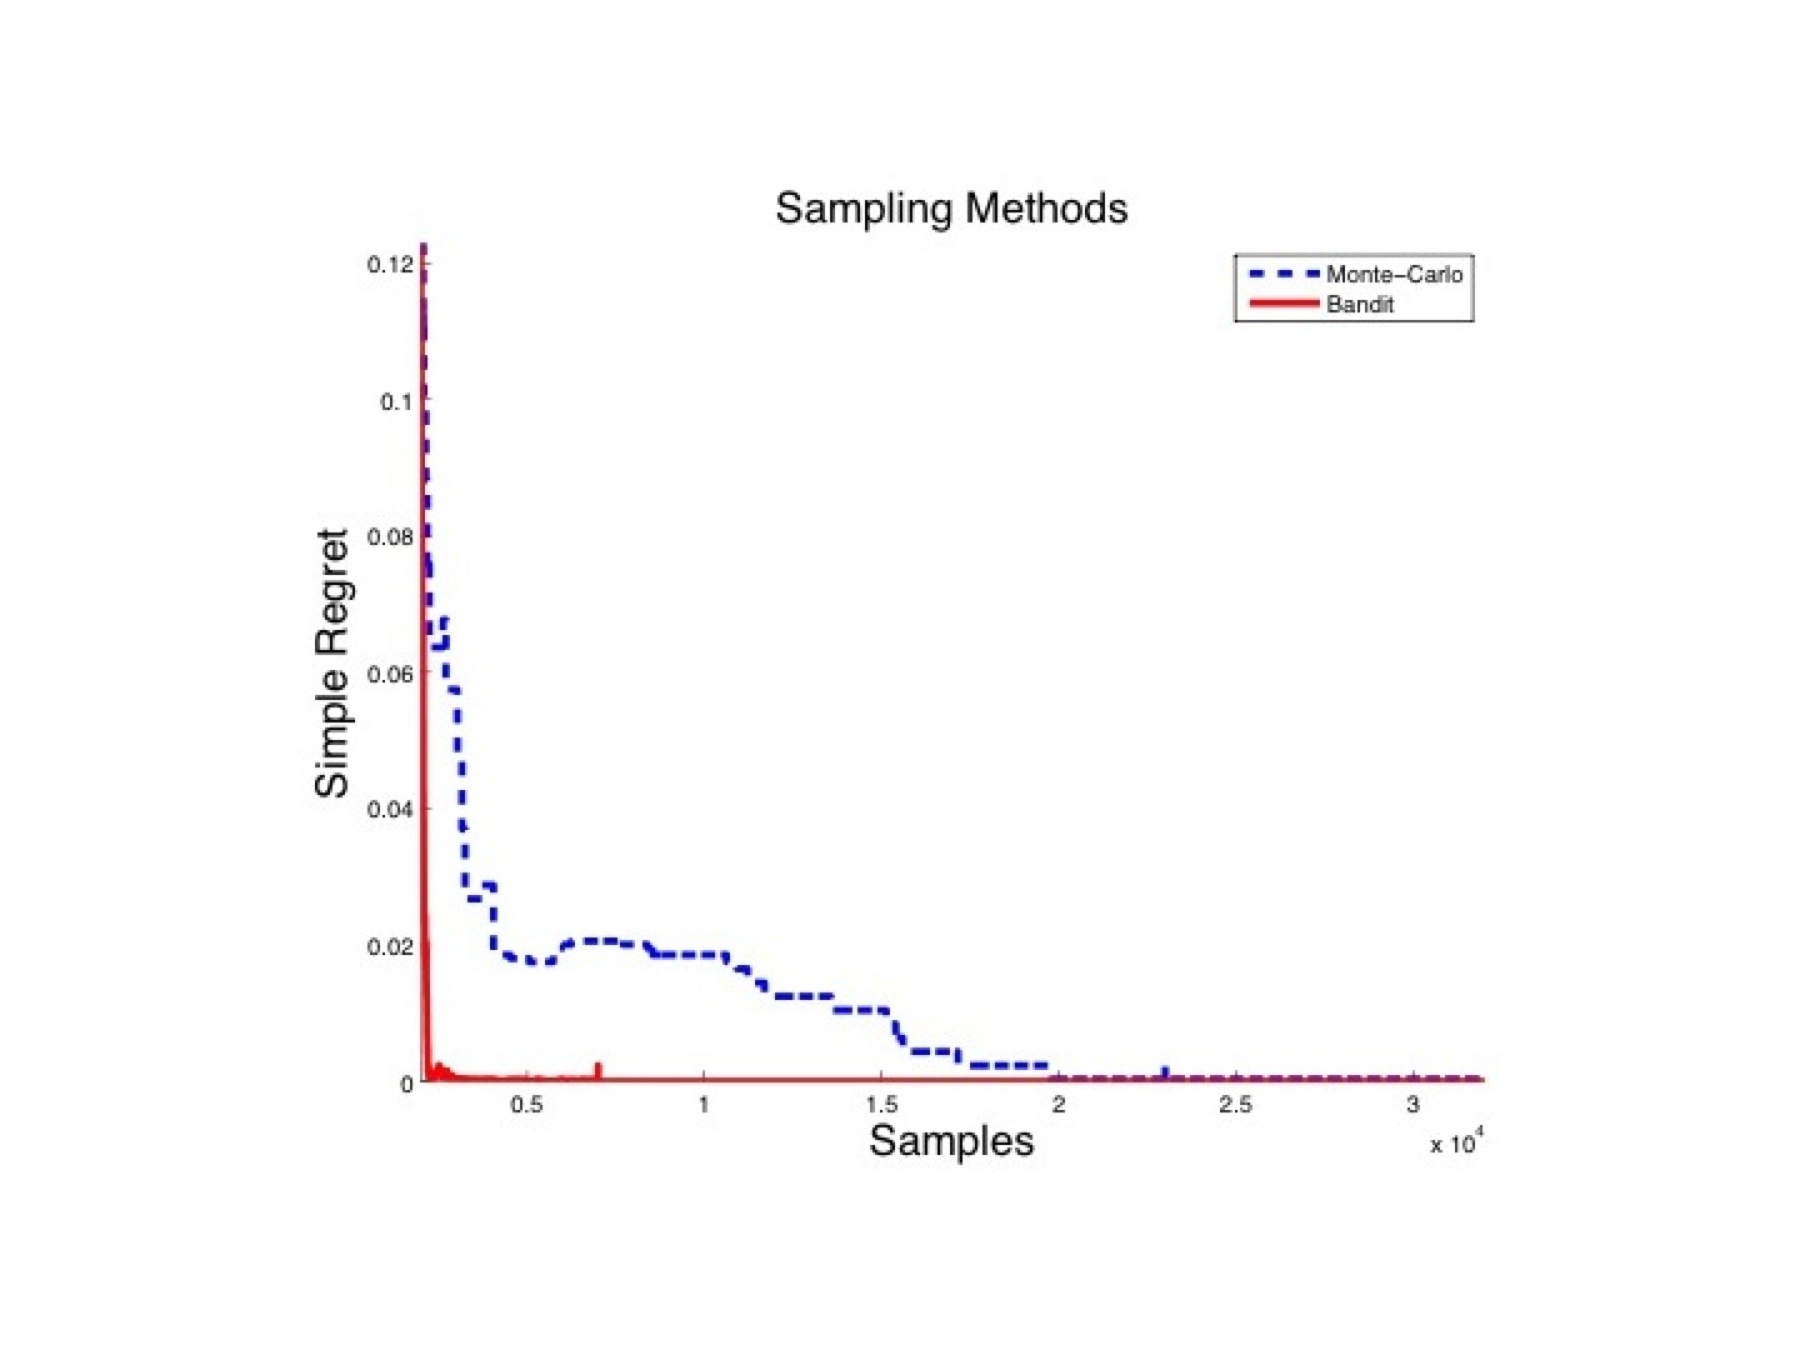
\includegraphics[width = 6cm, height = 4cm]{figures/Slide01.jpg}
\caption{Illustration of a grasp plan $\Gamma$ composed of two lines of action, $\gamma_1(t)$ and $\gamma_2(t)$}
\vspace*{-10pt}
\label{fig:line_of_action}
\end{figure}

\subsection{Types of Uncertainty}
In this work we consider the following types of uncertainty shape, pose, movement, and friction coefficient.  The property of force closure is not affected by the center of mass because it  measures if a wrench can be resisted not how large the force is need to resist.  Fig. \ref{fig:graphical_model} shows the probabilistic relationship of the types of uncertainty considered in this work. We model each one of these with a corresponding distribution and demonstrate how MAB algorithms can handle the types of uncertainty. We note though that our choice of distributions does not effect the ability to use the MAB algorithms and that the reader should choose distribution that effect their needs. 

\subsubsection{Distribution on Shape}

Shape uncertainty can occur from transparency, occlusions and sensor noise \cite{mahler}. To model this uncertainty we use a Gaussian Process Implicit Surface (GPIS) representation, which is explained in detail in Appendix \ref{sec:Appendix}.  A GPIS is a Gaussian distribution on a signed distance function,$sd$, that describes the workspace. A signed distance function is  greater than 0 outside the surface of an object, 0 at the surface and less than 0 beneath.  Signed distance functions can be sampled from  $N(\mu(x),\Sigma(x))$, where $\mu(x)$ and $\Sigma(x)$ are the mean and covariance functions of the GPIS. For our application, we set $x$ to discretized points along the workspace $\mathcal{W}$ and for each sample the points that correspond to zero, $sd(x) = 0$, are the contours of the shape. For convenience we will  represent the $\mu(x)$ and $\Sigma(x)$ as the tuple $\theta = \left( \mu(x), \Sigma(x) \right)$. 

\subsubsection{Distribution on Pose}
In typical robotics applications the pose of objects in the envinroment is determined by registering the object frame-of-reference to the control frame-of-reference used for grasp execution.
Therefore pose uncertainty may come from two primary sources a) uncertainty about the registration of the robot's grasping frame-of-reference to its sensing frame-of-reference and b) uncertainty about the pose of known object models in the robot's sensor data.
The effects of pose uncertainty on robotic grasping has been studied by ~\cite{}.

The pose of an object $T$ is a member of the Lie Algebra $SE(3)$ in 3-dimensional space (something analogous holds for 2D).
This matrix is defined by 3 rotation angles $\bw = (\alpha, \beta, \gamma)$ and 3 translation coordinates $\bt = (t_x, t_y, t_z)$, summarized in parameter vector $\mathbf{\xi} = (\bw, \bt)^T \in \mathbb{R}^6$.
One challenge with pose is that uncertainty in the pose matrix $T$ used to apply transformations is needed in practice, but uncertainty is mathematically more easily to quantify in terms of the pose parameters $\xi$.
Thus given a mean pose matrix $\bar{T} \in SE(3)$ and zero-mean uncertainty on the pose parameters $\mathbf{\xi} \sim \mN \left( \mathbf{0}, \Sigma \right)$ we define the pose random variable $T$ as

\vspace{-2ex}
\begin{align*}
	T  &= \exp \left( \mathbf{\xi}^{\wedge} \right) \bar{T}
\end{align*}

\noindent where the $\wedge$ operator is defined as in \cite{barfoot2014Pose}.

 
 \subsubsection{Distribution on Motion}
 In practice a robot may not be able to execute a desired
grasp plan $\Gamma$ exactly due to errors in trajectory following or
registration to the object \cite{kehoe2012estimating}. To handle this uncertainity, we sample the angle of approach $\rho$ of the proposed grasp plan $\Gamma$ from a zero mean one-dimensional Guassian $\rho \sim N(0,\sigma_{mot}^2)$. In practice $\sigma_{mot}^2$ might be set from repeatibility measurements for a robot \cite{mooring1986determination}.

 
 \subsubsection{Distribution on Friction Coefficient}
As shown in \cite{zheng2005}, uncertainty in friction coefficient can play a large role in grasp quality evaluation. The expected friction coefficient $E(\mu)$ can be derived by means of object classification and a look up table. However, because their could be material in between the objects surface and the robot gripper (i.e. dust, water, moisture), we purpose sampling the friction coefficient from a Gaussian around the expected friction coefficient $\mu \sim N(E(\mu),\sigma_{\mu}^2)$. 
 
 
To estimate $P(Q(\Gamma)>0)$, we sample from the graphical model shown in Fig. \ref{fig:graphical_model}. To sample from $p(Q(\Gamma)>0)$, we need to sample from the distributions associated with a line of action $p(\textbf{n}_i,\textbf{c}_i|\gamma_i(t),\xi,\theta, \rho)$. Using Bayes rule  we can rewrite this as 
 
 \vspace{-2ex}
 \begin{align*}
 &p(\textbf{n}_i,\textbf{c}_i |\gamma_i(t),\theta,\xi,\rho)=\\
 &p(\textbf{n}_i|\textbf{c}_i,\theta)p(\textbf{c}_i|\gamma_i(t),\theta,\rho,\xi)
 \end{align*}
 
 Appendix \ref{sec:Appendix}, describes how to draw shape sample from a GPIS model, which is used to compute $p(\textbf{c}_i|\gamma_i(t),\theta,\rho,\xi)$ along with the other sampled distribution on pose ($\xi$) and motion ($\rho$). Appendix \ref{sec:normals}, describes how to sample from $p(\textbf{n}_i|\textbf{c}_i,\theta)$ and presents a novel visualization technique for the distribution on surface normals.  Appendix \ref{sec:mass}, describes a way to calculate the expected center of mass assuming a uniform mass distribution. 
 
 



\begin{figure}[ht!]
\centering
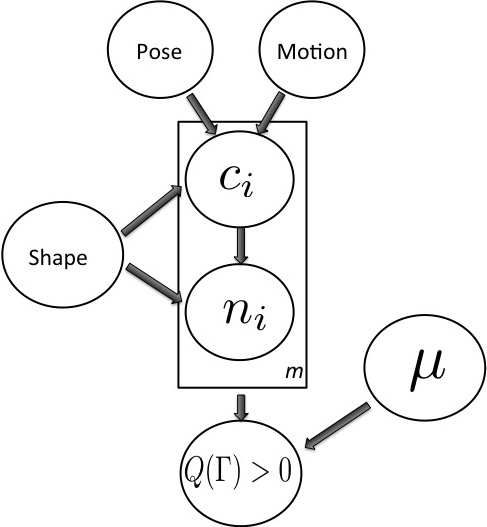
\includegraphics[width = 6cm, height = 6cm]{figures/Slide8.jpg}
\caption{A graphical model that illustrates the relationship between the different types of uncertainty in an object. Center of Mass uncertainty is dependent on the pose and shape of the object, however friction coefficient is independent of all other types. \todo{Should we use words or symbols for the graphical model?}}
\vspace*{-10pt}
\label{fig:graphical_model}
\end{figure}





\subsection{Problem Definition}

We assume we are given a 2-D workspace $\mathcal{W}$ with an unknown object represented as a trained GPIS model, described in Section \ref{sec:GP}, and set of possible grasp plans $G$ which are generated either uniformly randomly or with a heuristic as in \cite{mahler2015gp}.
We are interested in determining Eq. \ref{eq:problem_def} with respect to the problaliltiy of achieving force closure or $P(Q(\Gamma) > 0)$. \todo{Need to figure out if we can use optimal or not}

\vspace{-2ex}
\begin{align}\label{eq:problem_def}
\Gamma^* \in \underset{\Gamma \in G}{\mbox{argmax}} P(Q(\Gamma)>0)
\end{align}





\section{Multi-Armed Bandits for Grasp Selection}
While a standard approach to solving the problem in Eq. \ref{eq:problem_def} would be to perform Monte-Carlo integration on each $\Gamma_i$ and compute the probability of force closure, we propose treating the problem as a multi-armed bandit model and forming a policy for selecting which grasp to sample. The multi-armed bandit model, originally described by Robbins \cite{robbins1985some}, is a statistical model of an agent attempting to make a sequence of correct decisions while concurrently gathering information about each possible decision. Solutions to the multi-armed bandit model have been used in applications for which evaluating all possible options is expensive or impossible, such as the optimal design of clinical trials~\cite{simon1989optimal}, market pricing~\cite{rothschild1974two}, and choosing strategies for games~\cite{st2012online}. 

The traditional setting of a multi-armed bandit model is a gambler that has K independent slot machine arms and decides what machines to play, how many times to play each one, what order to play them in.
A successful gambler would want to exploit the machine that currently yields the highest reward and explore new arms to see if they give better rewards.
Developing a policy that successfully trades between exploration and exploitation has been the focus of extensive research since the problem formulation \cite{bubeck2009pure}, \cite{robbins1985some}, \cite{bergemann2006bandit}.

In our setting, we have a probabilistic  representation and would like to evaluate many potential grasps on the samples drawn from the graphical model in Fig. \ref{fig:graphical_model}.
Motivated by limited computational resources we  allocate sampling resources to efficiently find the best arm.
Here each arm corresponds to a different grasp plan and pulling the arm is sampling from the graphical model in Fig. \ref{fig:graphical_model} and evaluating the arm's grasp plan on the sample.



A common measure of success in MAB problems is {\it regret}, the difference between the expected optimal reward and the expected reward of the selected arm on a single pull.
Traditional bandit algorithms minimize cumulative regret,  the sum of regret over the entire sequence of arm choices. Lai and Robbins showed that an optimal solution to the bandit problem is bounded by a logarithmic function \cite{lai1985asymptotically}. They presented an algorithm called (Upper Confidence Bound) UCB that obtains this bound asymptotically. Many variants of UCB have thus been proposed. The algorithm maintains a confidence bound on the distribution of reward based on prior observations and pulls the arm with the highest upper confidence bound. 


In the context of finding a high quality grasp, one only cares about the regret when the grasp is actually executed in real life. The agent shouldn't be penalized for exploring different grasps, but only for the grasp that they suggest at the termination of the algorithm. Hence, the exploration and exploitation stage are decoupled. Our goal is to identify the best arm in as few decisions as possible.
Given a set of arms $\lbrace 1,...K \rbrace$ with respective mean rewards $\mu_1, ..., \mu_K$ and the optimal arm $\mu^* = \underset{k\in\lbrace 1, ..., K \rbrace}{\mbox{max}} \mu_k$.
The simple regret at time $t$ is given by

\vspace{-2ex}
\begin{align}\label{eq:simple_regret}
r_t = \mu^* - \mu_t
\end{align}
\noindent where $\mu_t$ is the estimate of the best arm at time $t$ from the previous observations. 

Best arm identification has a wide variety of literature that largely falls into two camps: one where the algorithm terminates once a fixed confidence interval around the best arm is met and the Budgeted Multi-Armed Bandit (BMAB) model, in which the algorithm must make a decision at the end of a fixed ``budget'' number of arm pulls.

\subsection{Fixed Confidence}
In the fixed confidence setting the forecaster seeks to minimize the simple regret until a fixed confidence threshold is met at which point it terminates. Originally the problem was solved with `racing' algorithms, which used Hoeffding inequalities or the empirical Bernstein inequality to prune arms that were likely to be suboptimal and used uniform allocation to explore the remaining set \cite{maron1993hoeffding} \cite{mnih2008empirical}. These methods were later extended to return the top $m$ arms instead of only the best arm\cite{gabillon2012best}. 

The speed of termination is affected by the hardness of the problem, which relates to the how close the other arms expected reward is to the expected reward top arm in the set \cite{audibert2010best}. In the grasping context this means that achieving a fixed confidence for two similar grasps would require exhaustive sampling from each distribution. 

\subsection{Fixed Budget}

In the Budgeted Multi-Armed Bandit (BMAB) setting the algorithm is given a stopping time and needs to return the current best arm at that stopping time this can be thought of as an anytime algorithm.   Audibert el al. demonstrated an algorithm called Successive Rejects that divides up the total budget into successively shorter phases and discards the worst arm left at the end of each phase. This algorithm can return the best arm with near-optimal probability depending on the hardness of the problem \cite{audibert2010best}. In addition, UCB-like methods have been proposed that measure a confidence gap and then pull the arm with the highest confidence interval \cite{gabillon2012best}. For example in \cite{bubeck2009pure}, they showed a link between simple regret and cumulative regret that allowed for the analysis of the existing bandit algorithms like UCB1.

In this work, we consider a setting in which a robot has a fixed computational time limit to select a grasp and thus the fixed budget setting is more appropriate. The time limit can be chosen via repeatibility experiments on a desire task. In Section \ref{sec:bandit_algorithm}, we will discuss some of the specific budgeted multi-armed bandit algorithms that are used in practice. 


\section{Bandit Algorithms For Best Arm Identification}\label{sec:bandit_algorithm}


While, UCB type algorithms adopt a frequenist perspective for distributions with bounded rewards in their empirical estimate of an upper bound. A growing interest though in the MAB community is in bandit algorithms that have Bayesian approach \cite{kaufmann2012bayesian} \cite{agrawal2011analysis}. Here a prior distribution is placed on the distribution to be estimated and utilizing the prior enables a trade off between exploration and exploitation. Theoretical results have shown that these methods are capable of achieving the lower bound described by Lai and Robbin \cite{agrawal2011analysis} \cite{kaufmann2012bayesian}. Furthermore in an empirical study Bayesian methods have been shown to outperform the UCB family \cite{chapelle2011empirical}.  

In the context of grasping, the reward from sampling from the grasp distribution is 1 if the sampled grasp is in force closure and 0 if the grasp is not in force closure. The distribution that describes whether an event is $\lbrace 0, 1 \rbrace$ is known as a Bernoulli distribution and can be described by the parameter $\theta$ or the probability an event occurs. In the Bayesian setting one would treat $\theta$ as belonging to a distribution. A convenient and common choice for such a distribution is the Beta distribution. Beta distributions are specified by shape parameters $\alpha$ and $\beta$, where ($\alpha >0$ and $\beta >0$). The mean of the Beta distribution is given by $\alpha/(\alpha+\beta)$. To update the prior Beta distribution one simply adds the count of observed successes of the event to $\alpha$ and the count of the observed failures to $\beta$. The default $\alpha =1 $ and $\beta =1$ corresponds to a uniform distribution on $\theta$. 

Given a proposed grasp plan $\Gamma$ , we draw samples from the shape distribution $P (\theta )$, the distribution on pose $P (\xi)$, distribution on motion $p(\rho)$ and the distribution on friction coefficient $P (\mu)$. The distribution on force closure can then be estimated as Beta- Bernoulli Process with shape parameters $\alpha$ and $\beta$. Thus, we can write the expected probability of force closure as follows


\vspace{-2ex}
\begin{align}\label{eq:shape_sampling}
P(Q(\Gamma|\theta,\mu,\xi,\rho) > 0) = \frac{\alpha}{\alpha + \beta}
\end{align}

Where $Q(\Gamma|\theta,\xi,\mu,z)$ is the grasp quality that is computed on a shape sample drawn from $p(\theta)$,$p(\xi)$,$p(\rho)$ and $p(\mu)$. Whats interesting in the context of a Bayesian BMAB problem our  graphical model in Fig. \ref{fig:graphical_model}, is now equivalent in terms of inference to \ref{fig:beta_model} and we only need to estimate $\alpha$ and $\beta$ to determine grasp quality. Regardless of the distributions in Fig. \ref{fig:graphical_model}, we are still able to maintain the theoretical guarantees given by the Bayesian MAB algorithms because the probability of force closure is a Beta-Bernoulli Process \cite{agrawal2011analysis} \cite{kaufmann2012bayesian} \cite{weber1992gittins}.  

\begin{figure}[ht!]
\centering
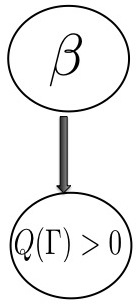
\includegraphics[width = 2cm, height = 4cm]{figures/Slide9.jpg}
\caption{A graphical model that illustrates the relationship between the Bernoulli distribution of the probability force closure and its conjugate prior Beta distribution that has two shape parameters $\alpha$ and $\beta$ }
\vspace*{-10pt}
\label{fig:beta_model}
\end{figure}


%In practice, when the distribution on the rewards of arms is not known, the empirical methods such as $\epsilon-$greedy have shown to have better performance in some situations \cite{kuleshov}.

%In our case we only care about the regret at the time our decision of the optimal grasp needs to be made, decoupling the exploration and exploitation stages.



\subsection{Bayes-UCB}
Bayes UCB, detailed in Algorithm 1, is a version of the UCB algorithm that uses a Bayesian posterior update to get a confidence bound instead of  the frequentist concentration inequality approach. To get an upper confidence bound from the posterior, the Bayes UCB algorithm uses the quantile of the Beta distribution up to a specified probability which depends on the timestep and horizon. TAt each time step the arm with the highest quantile is chosen and the Beta distribution is updated based on the observed reward.  For binary rewards (i.e. Bernoulli distributions) the expected number of pulls of suboptimal arms is bounded and experimentally this algorithm has been shown to outperform UCB for binary rewards \cite{kaufmann2012bayesian}.

\begin{algorithm}
 \KwResult{Current Best Arm, $\Gamma^*$ }
 For Beta(1,1) prior, Stopping Horizon $n$: \\
\For{ t=1,2,...,n}{ 
	\For{j = 1,...,K}{
	
		Compute: $q_j(t) = Q\big(1-\frac{1}{t},p_j^{t-1}\big)$
	
	}
Draw arm$ I_t = \mbox{argmax}_{j=1...K}q_j(t)$\\
 Observe reward $X_{I_t,t} \in \lbrace 0,1 \rbrace$\\
 Update posterior:\\
 Set $S_{I_t,t+1} = S_{I_t,t} + X_{I_t,t}$ \\
 Set $F_{I_t,t+1} = F_{I_t,t} + 1 - X_{I_t,t}$\\
 Set $\theta_j^t \sim \mbox{Beta}(S_{I_t,t+1},F_{I_t,t+1} )$\\
 }
 \caption{Bayes-UCB for Beta-Bernoulli Process}
\end{algorithm}


\subsection{Thompson Sampling}
Thompson Sampling is a Bayesian method for the multi-armed bandit problem. We will describe it now in detail for the Beta-Bernoulli process. All arms are initialized with a prior Beta distributions, which is normally Beta($\alpha=1$,$\beta =1$) to reflect a uniform prior on the $\theta$ of the Bernoulli distribution. Then for each arm draw $\theta_{j,t} \sim \mbox{Beta}(\alpha,\beta)$ and pull the arm with the highest $\theta_{j,t}$ drawn. The reward, $X_{i,t}$ is observed from that arm, $j$, and the corresponding Beta distribution is updated. This is repeated until a stopping time is reached. The full algorithm is shown in Algorithm 1.  

The randomness of Thompson sampling allows for it to quickly explore the more arms then Bayes-UCB, which makes conservative arm pulls based on confidence bounds. It is also less prone to local solutions because of its stochastic nature. Thus, for cases where exploration and exploitation are decoupled Thompson sampling can find a better arm faster. Thompson sampling has recently been shown to approach the Lai and Robbins bound \cite{agrawal2011analysis} and has  empirically been shown to outperform frequentist methods like UCB in certain settings \cite{chapelle2011empirical}. Variants of it are even used commercially in products like Microsoft's adPredictor, which is used by Bing, the search engine, \cite{graepel2010web}. 
\begin{algorithm}
 \KwResult{Current Best Arm, $\Gamma^*$ }
 For Beta(1,1) prior: \\
\For{ t=1,2,...}{ 
 Draw $\theta_{j,t} \sim$ Beta($S_{j,t}+1$,$F_{j,t}+1$) for $j = 1,...,k$\\
 Play $I_t=j$ for $j$ with maximum $p_{j,t}$\\
 Observe reward $X_{I_t,t} \in \lbrace 0,1 \rbrace$\\
 Update posterior:\\
 Set $S_{I_t,t+1} = S_{I_t,t} + X_{I_t,t}$ \\
 Set $F_{I_t,t+1} = F_{I_t,t} + 1 - X_{I_t,t}$\\
	
 }
 \caption{Thompson Sampling for Beta-Bernoulli Process}
\end{algorithm}



\subsection{The Gittins Index Method} 
\todo{Let me know how clear this is, Gittins can be hard to describe in general}
One possible solution to solve the MAB problem is to treat it as an Markov Decision Process (MDP) and use Markov Decision theory. This solution makes a lot of sense when the distribution is known because the all elements in the standard MDP tuple, $\lbrace S,A,T,R,\gamma \rbrace$, would be known and it is optimal with respect $\gamma$ \cite{weber1992gittins}. 

However, the curse of dimensionality effects performance because if you have $K$ arms, a finite horizon of $T$ and a Beta-Bernoulli distribution on your arms then your state space is on the order of $T^{2*K}$. Hence the complexity of solving MAB using Markov Decision theory increases exponentially with the number of bandit processes. A key insight though was given by Gittins, who showed that instead of solving the $k$-dimensional MDP one can instead solve $k$ 1-dimensional optimization problems: for each arm $i$, $i= 1,...,k$, and for each state of $x^i = \lbrace \alpha_0 +S_t, \beta_0 +F_t \rbrace^i$, where $S_t$ and $F_t$ correspond to the number of success and failures at pull $t$. 


\vspace{-2ex}
\label{eq:git_indices}
\begin{align}
	v^i(x^i) = \underset{\tau>0}{\mbox{max}} \frac{\mathcal{E}[\sum_{t=0}^{\tau}\gamma^tr^i(X_t^i)|X_0^i = x_i]}{\mathcal{E}[\sum_{t=0}^{\tau}\gamma^t|X_0^i = x_i]}
\end{align}


The indices can be considered as a computation of the value in choosing an arm conditioned on the fact that you will give up an choose another arm at some point. Once you know the state of your $k$ arms, the algorithm is to select the one with the highest index.  For Best Arm Identification you want your discount factor $\gamma$ to approach 1, since you should never stop pulling the best arm. Generally the computation of the Gittins indices is too expensive, however in the Beta-Bernoulli case it is actually possible \cite{kaufmann2012bayesian}. We computed the Gittins indices offline using the restart method proposed by Katehakis et al. \cite{katehakis1987multi}.


\begin{algorithm}
 \KwResult{Current Best Arm, $\Gamma^*$ }
 For Beta(1,1) prior, Table of Indices $v$, Discount Factor $\gamma$: \\
\For{ t=1,2,...}{ 
 Pull arm $k = \underset{x_k \in X}{\mbox{argmax}} v(x_k)$\\
 Observe reward $R_{I_t,t} \in \lbrace 0,1 \rbrace$\\
 Update posterior:\\
 Set $S_{I_t,t+1} = S_{I_t,t} + R_{I_t,t}$ \\
 Set $F_{I_t,t+1} = F_{I_t,t} + 1 - R_{I_t,t}$\\
 Set $x_k = \lbrace 1 + S{I_t,t+1}, 1+F_{I_t,t+1} \rbrace$\\	
}
 \caption{The Gittins Index Method for Beta-Bernoulli Process}
\end{algorithm}

 .
\section{Experiments}
For the experiments we used the Brown Vision Lab 2D dataset, the same used in \cite{christopoulos2007handling}. We downsampled the image by a factor of 2 to create a 40 x 40 occupancy map, which holds 1 if the point cloud was observed and 0 if it was not observed, and a measurement noise map, which holds the variance 0-mean noise added to the SDF values. The parameters of the GPIS were selected using maximum likelihood on a held-out set of validation shapes. The noise of the motion, position and friction coefficient was set to the following variances $\sigma_{mu} = 0.4$, $\sigma_{rot} = 0.3$ rads,$\sigma_{trans} = 3$. Our visualization technique follows the approach of \cite{mahler2015gp} and consisted of drawing many shape samples from the distribution and blurring accordingly to a histogram equalization scheme. 

We did experiments for the case of two hard contacts in 2-D, however our methods are not limited to this implementation. We drew random lines of actions $\gamma_1(t)$ and $\gamma_2(t)$ by sampling around a circle with radius $\sqrt{2}n$ and sampling the circles origin, then projecting onto the largest inscribing circle in the workspace. 

\subsection{Multi-Armed Bandit Experiments}
\todo{add Bayes and Kehoe results}
We consider the problem of selecting the best grasp plan, $\Gamma^*$ out of a set $G$. For our experiments we look at selecting the best grasp out of a size of $|G| = 1000$. In Fig. \ref{fig:simple_regret}, we plotted the simple regret averaged over 100 randomly drawn shapes in our data set and compare the different methods (UCB, Thompson, Gittins and the naive random allocation). We initialize both the Monte-Carlo and bandit technique by sampling each grasp 1 time. We draw samples from our calculated distributions $p(g)$.  Interestingly, Gittins and Thompson converge much faster than random and UCB. In Fig. \ref{fig:pulls_per_grasp}, you can see that Gittins and Thompson allocate grasp samples to only the grasps of high quality, thus they are quickly able to ignore the low quality grasps. UCB takes a more conservative approach to sample allocation, which leads to poor performance in the best arm identification problem \cite{bubeck2009pure}.

\begin{figure*}[ht!]
\centering
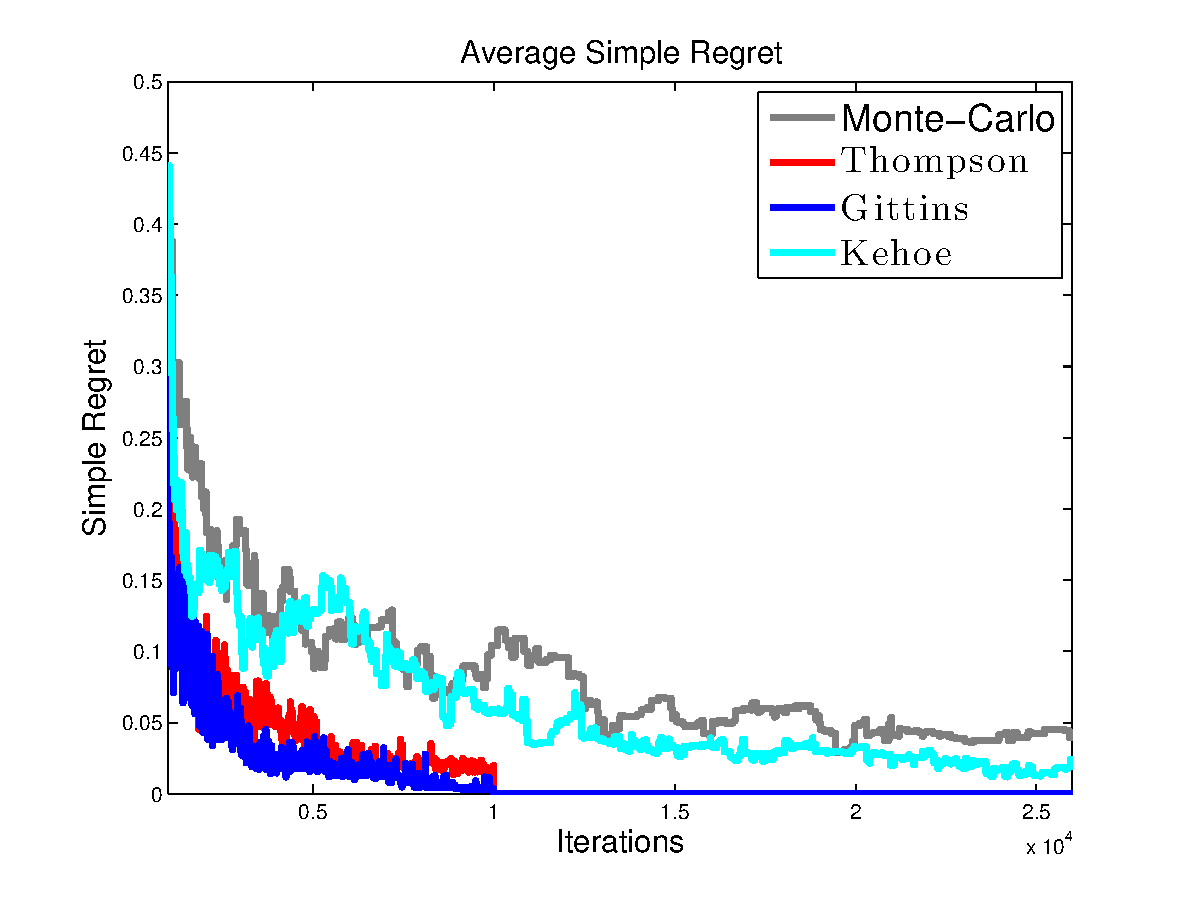
\includegraphics[width = 16.5cm, height = 9cm]{matlab_figures/simple_regret.eps}
\caption{ \footnotesize Comparison of Simple Regret convergence for the four sequential decision methods (Monte-Carlo, Bayes -UCB, Thompson, Gittins). Graph is averaged over 100 shapes from the Brown Sillohoute Dataset \cite{brown} with a set $|G|=1000$ for each shape. As you can see the BMAB methods converge almost a magnitude faster than random allocation. It is worth noting that Gittins outperform the other two algorithms, which is useful when choosing which one to implement }
\vspace*{-10pt}
\label{fig:simple_regret}
\end{figure*}


\begin{figure*}[ht!]
\centering
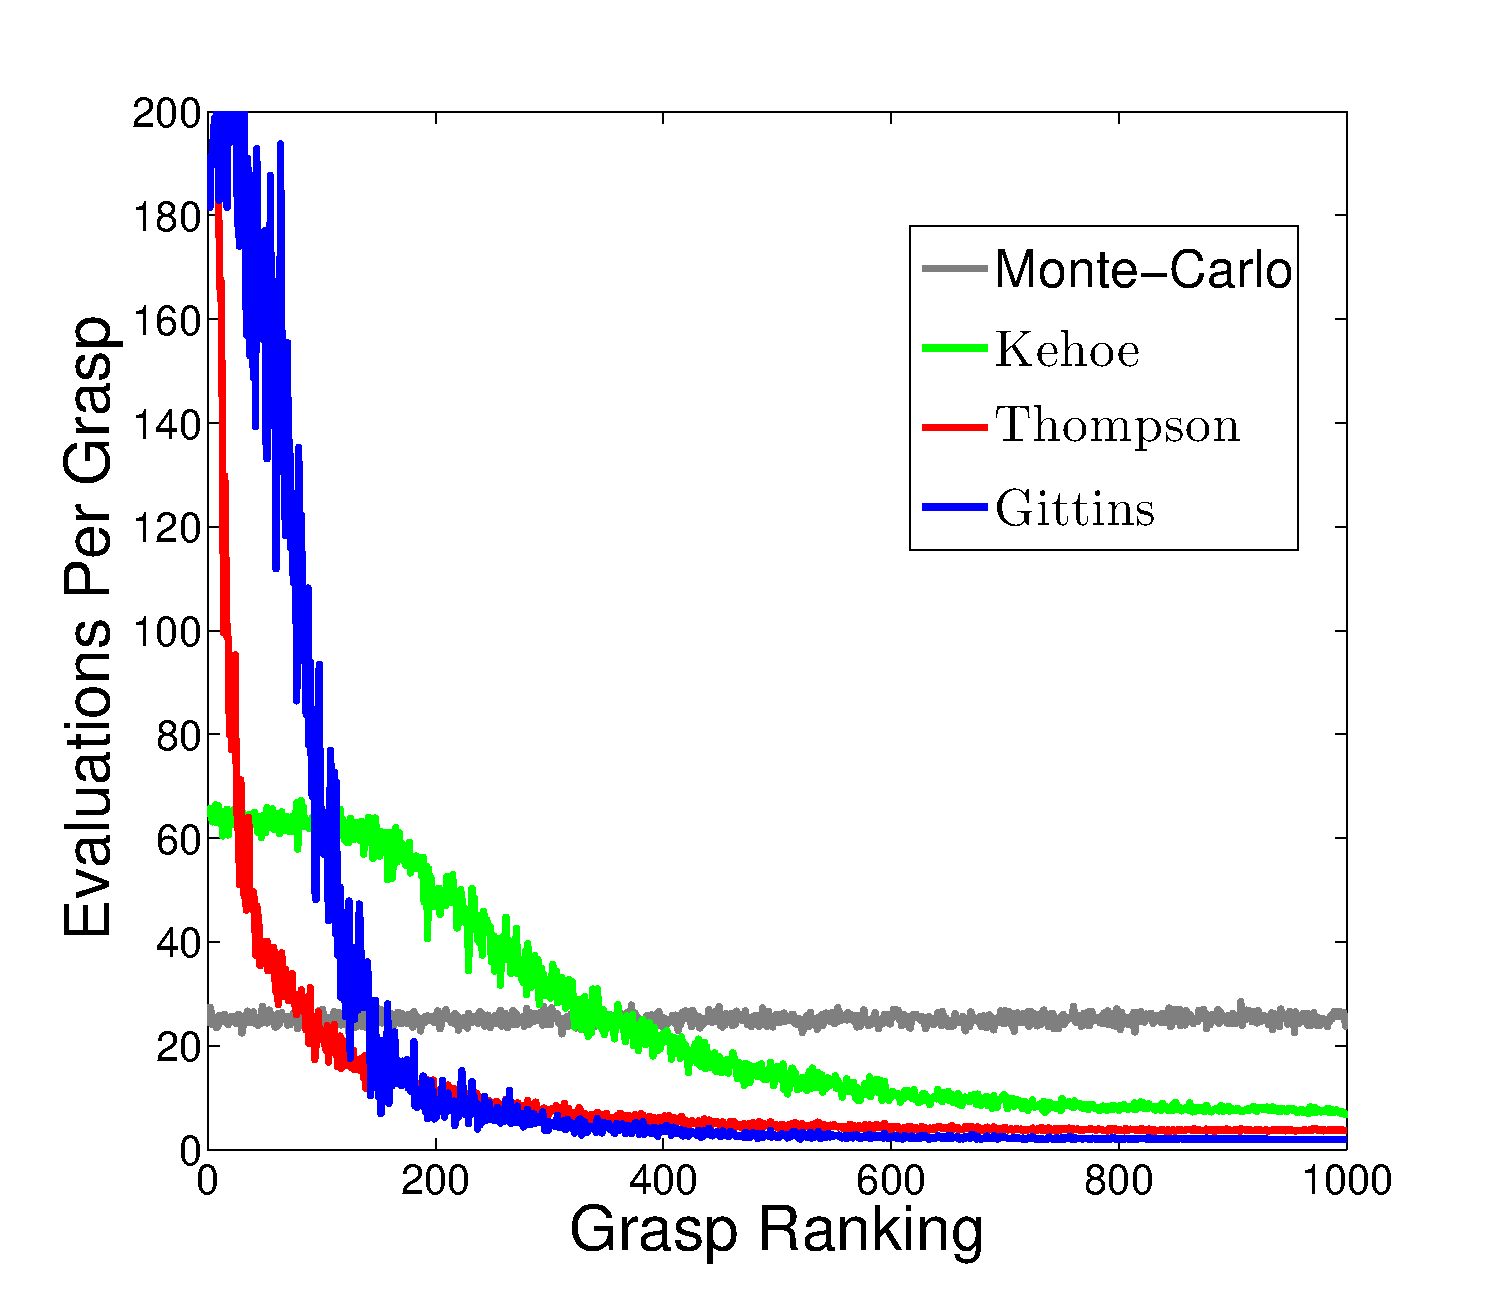
\includegraphics[width = 16.5cm, height = 9cm]{matlab_figures/pulls_per_grasp.eps}
\caption{ \footnotesize Comparison of sample per grasp for the four sequential decision methods (Random, Bayes - UCB, Thompson, Gittins). Graph is averaged over 100 shapes from the Brown Silhouette Dataset \cite{brown} with a set $|G|=1000$ for each shape. The best grasps are ranked 1 and worst are 1000. As you can see the MAB algorithm intelligently allocate samples towards high quality grasps based on past observations, where Monte-Carlo Integration takes a uniform approach to allocation. \cite{best_arm}}
\vspace*{-10pt}
\label{fig:pulls_per_grasp}
\end{figure*}
\begin{figure*}%
    \centering
    \subfloat{{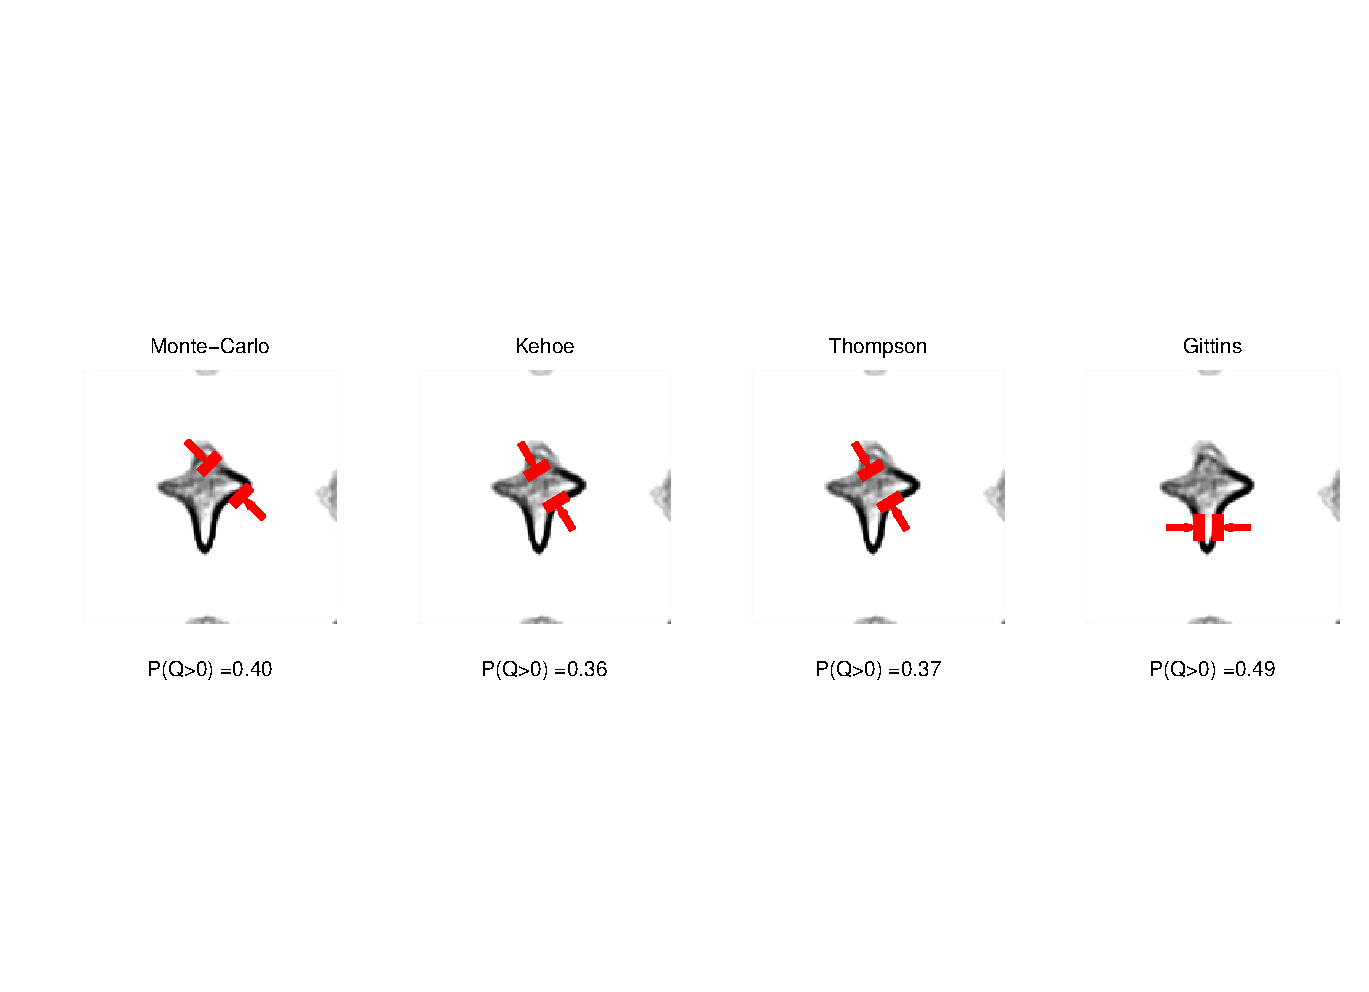
\includegraphics[width=16.5cm]{matlab_figures/shapes_1.eps} }}%
    \qquad
    \subfloat]{{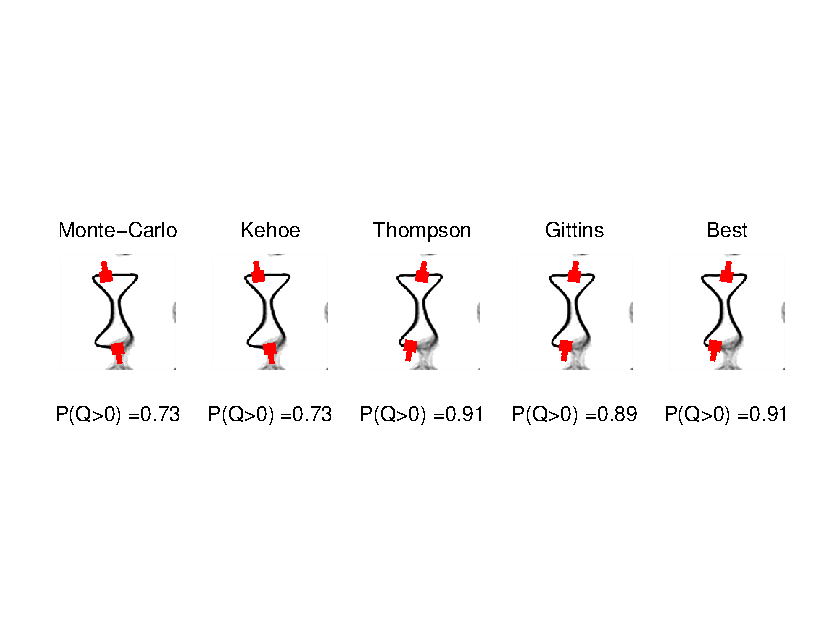
\includegraphics[width=16.5cm]{matlab_figures/shapes_2.eps} }}%
       \subfloat]{{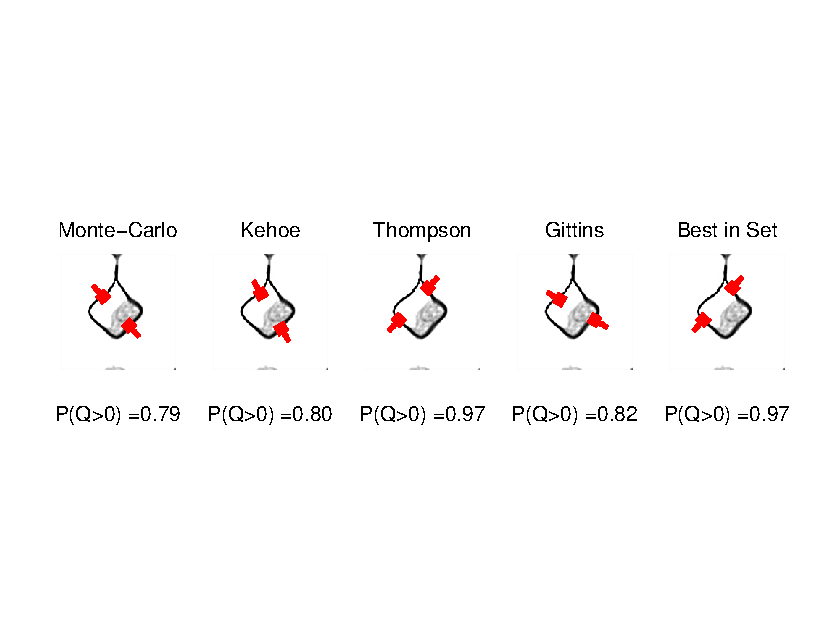
\includegraphics[width=16.5cm]{matlab_figures/shapes_3.eps} }}%
          \subfloat]{{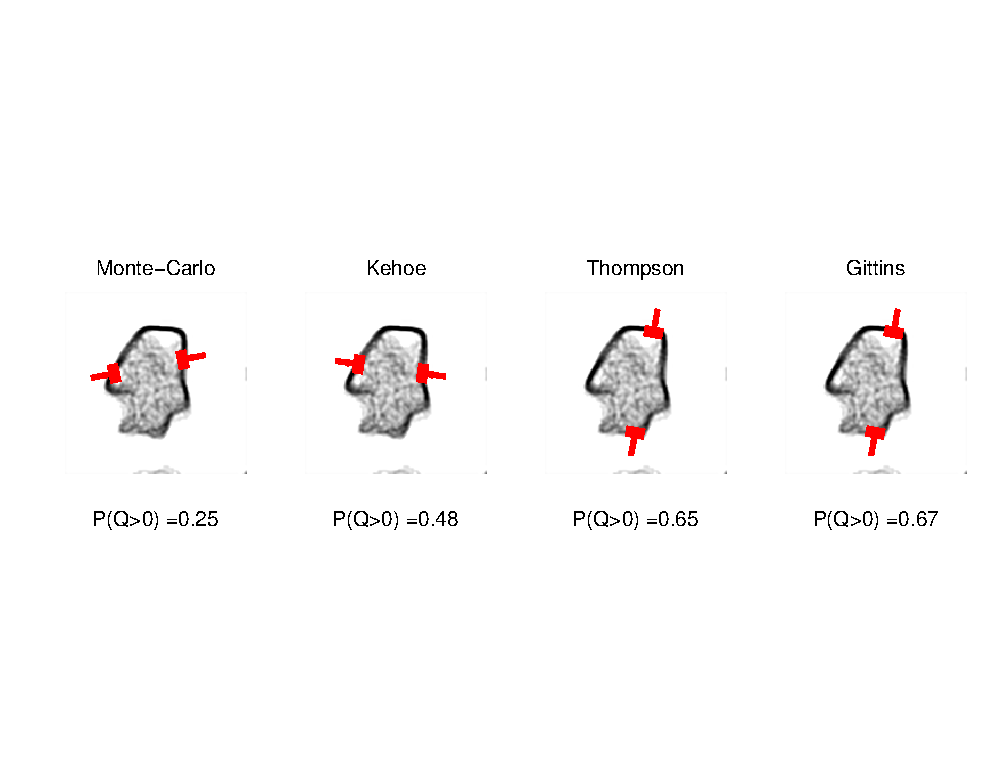
\includegraphics[width=16.5cm]{matlab_figures/shapes_4.eps} }}%
             \subfloat]{{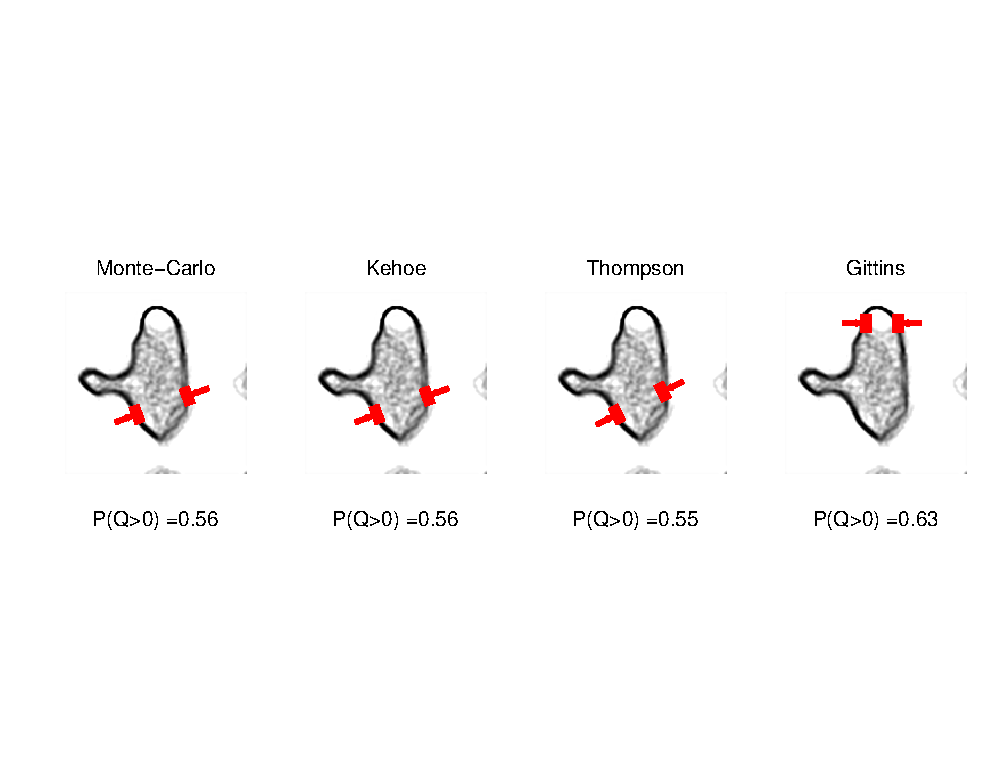
\includegraphics[width=16.5cm]{matlab_figures/shapes_5.eps} }}%
    
    \caption{Five shapes shown from the Brown Visual Lab Dataset with induced shape uncertainity and visualized according to the method described in \cite{mahler2015gp}. The four methods (Monte-Carlo, Kehoe's, Thompson and Gittins) were all run until a stopping time of 9000 evaluations with a uniformly initialized grasp set of $|G|=1000$. The grasps and the quality each one found is shown above. The Gittins Index Method in all cases shown found the best grasp among the methods.  }%
    \label{fig:rot_shapes}%
\end{figure*}

\subsection{Sensitivity Analysis }
We now will show how well the top two algorithms Thompson Sampling and the Gittens Index Method perform under a variation in noise from friction coefficient uncertainty, shape uncertainty, rotational pose and translation pose. The experiments are performed with the same setup as before but now we increase the variance parameters across a set range for each parameter to simulate low, medium and high levels of noise. All experiments were averaged across 10 shapes with a set size $|G| = 1000$. 

For friction coefficient we varied the variance across the following values $\sigma_{\mu} = \lbrace 0.05, 0.2, 0.4$. As illustrated in Fig. \ref{fig:fric_sens}, the performance of the bandit algorithm remains largely unchanged, with typical convergence to zero in simple regret less than 2000 evaluations.

For rotational uncertainity in pose, we varied $\sigma_{rot}$ over the set of $\lbrace 0.03, 0.12,0.24\rbrace$ radians. As you can see in Fig. \ref{fig:rot_sens}, the performance of the bandit algorithms is effected by the change in rotation, increase in variance to $0.24$ radians or $13^{\deg}$  causes the convergence in simple regret to not be reached until 5500 samples or an average of 5.5 samples per grasp. This can be explained because such a large variance causes a a drop in quality across all grasps and makes it harder to separate the outliers \cite{gabillon2012bes}. The quality of the best grasp along with the grasp for each round is shown in \ref{fig:rot_shapes}. 


For translational uncertainty in pose, we varied $\sigma_{trans}$ in the range of $\lbrace 3,12, 24 \rbrace$ units (on a 40 x 40 unit workspace). As you can see in Fig. \ref{fig:rot_sens}, the performance of the bandit algorithms is effected by the change in rotation, increase noise of $\sigma_{trans} = 24$ causes the convergence to not be reached until around 5000 samples for the Gittens Method and  8200 evaluations for Thompson Sampling.







\begin{figure}[ht!]
\centering
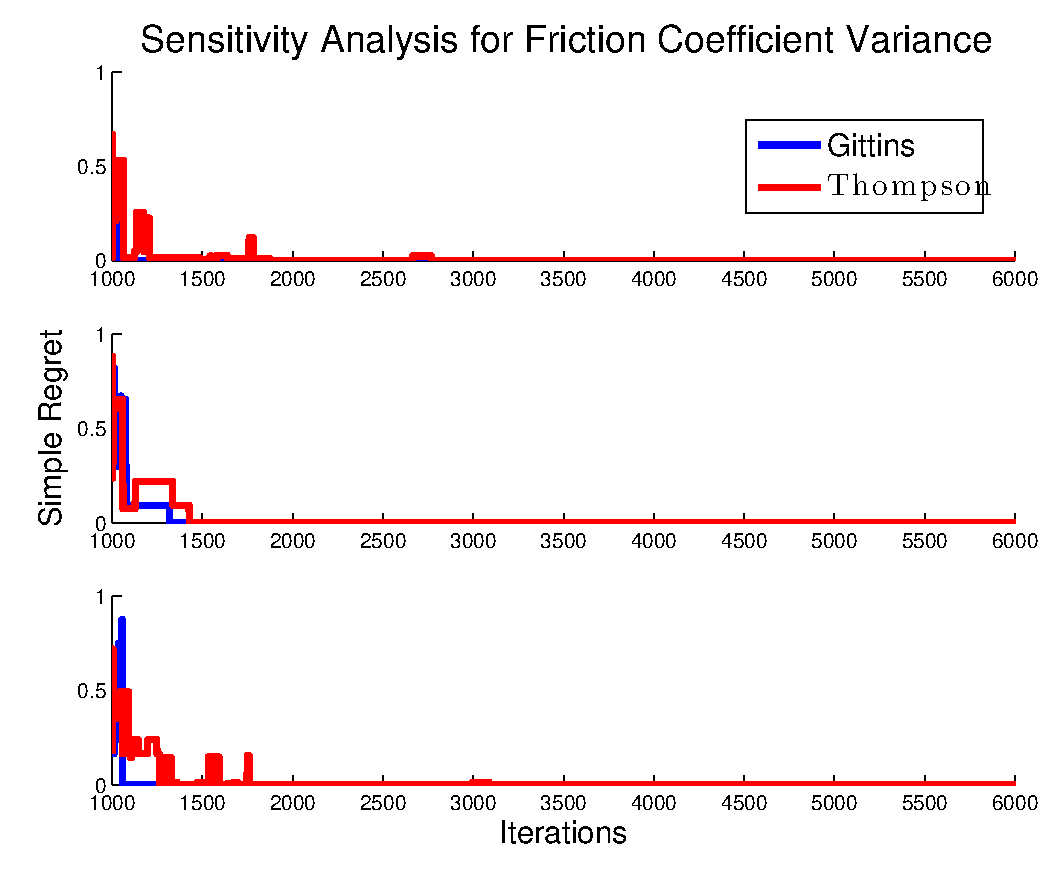
\includegraphics[width = 8cm, height = 10cm]{matlab_figures/sensitivity_fric.eps}
\caption{ \footnotesize Sensitivity Analysis for Thompson Sampling and the Gittens Index Method under friction coefficient uncertainty $\sigma_{fric} = \lbrace 0.05,0.2, 0.4 \rbrace$  from top to bottom on a 40 x 40 unit workspace averaged over 10 shapes from the Brown Vision Lab Data set. The increase in noise has little effect on the convergence of the two algorithms in simple regret.}
\vspace*{-10pt}
\label{fig:fric_sens}
\end{figure}

\begin{figure}[ht!]
\centering
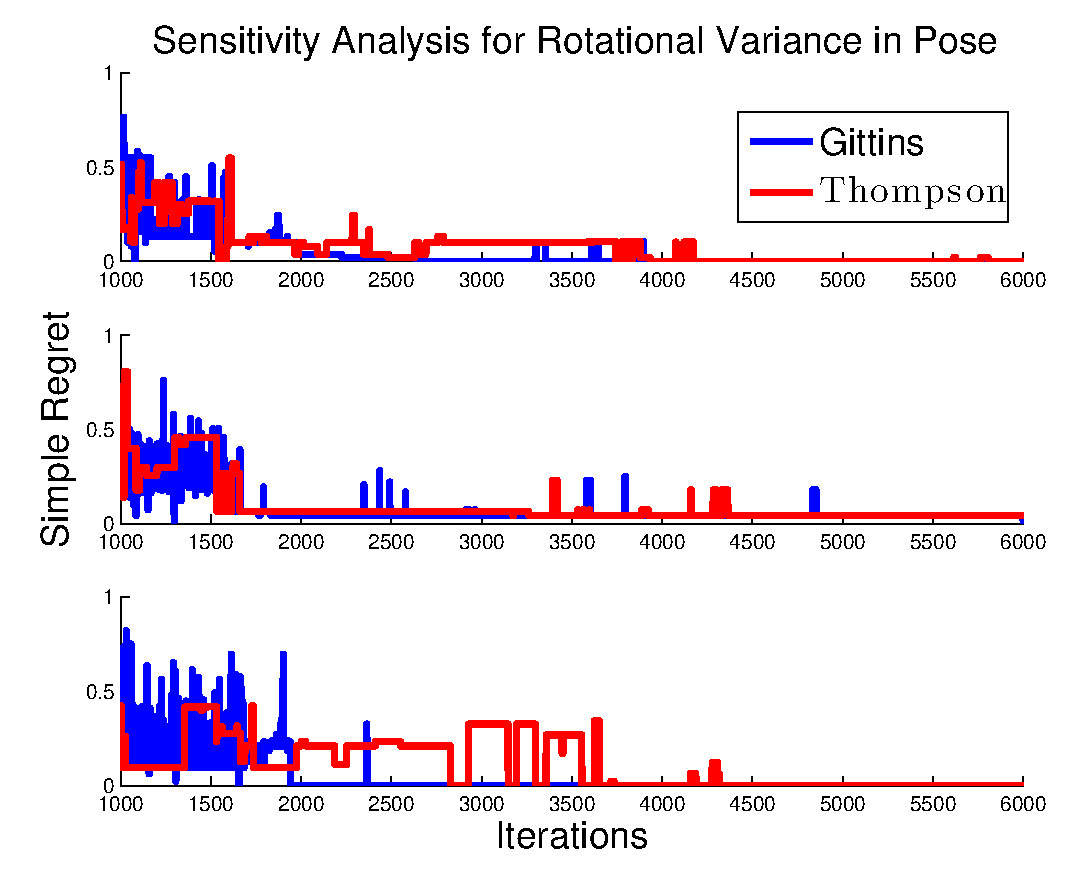
\includegraphics[width = 8cm, height = 10cm]{matlab_figures/sensitivity_rot.eps}
\caption{ \footnotesize Sensitivity Analysis for Thompson Sampling and the Gittens Index Method under coefficient of friction uncertainty $\sigma_{rot} = \lbrace 0.03,0.12, 0.24 \rbrace$ radians from top to bottom on a 40 x 40 unit workspace averaged over 10 shapes from the Brown Vision Lab Data set. The increase in noise has little effect on the convergence of the two algorithms in simple regret. \todo{Going to rerun with more shapes to be sure about this}}
\vspace*{-10pt}
\label{fig:rot_sens}
\end{figure}

\begin{figure*}%
    \centering
    \subfloat[lTop Grasps Shown for Shape 1]{{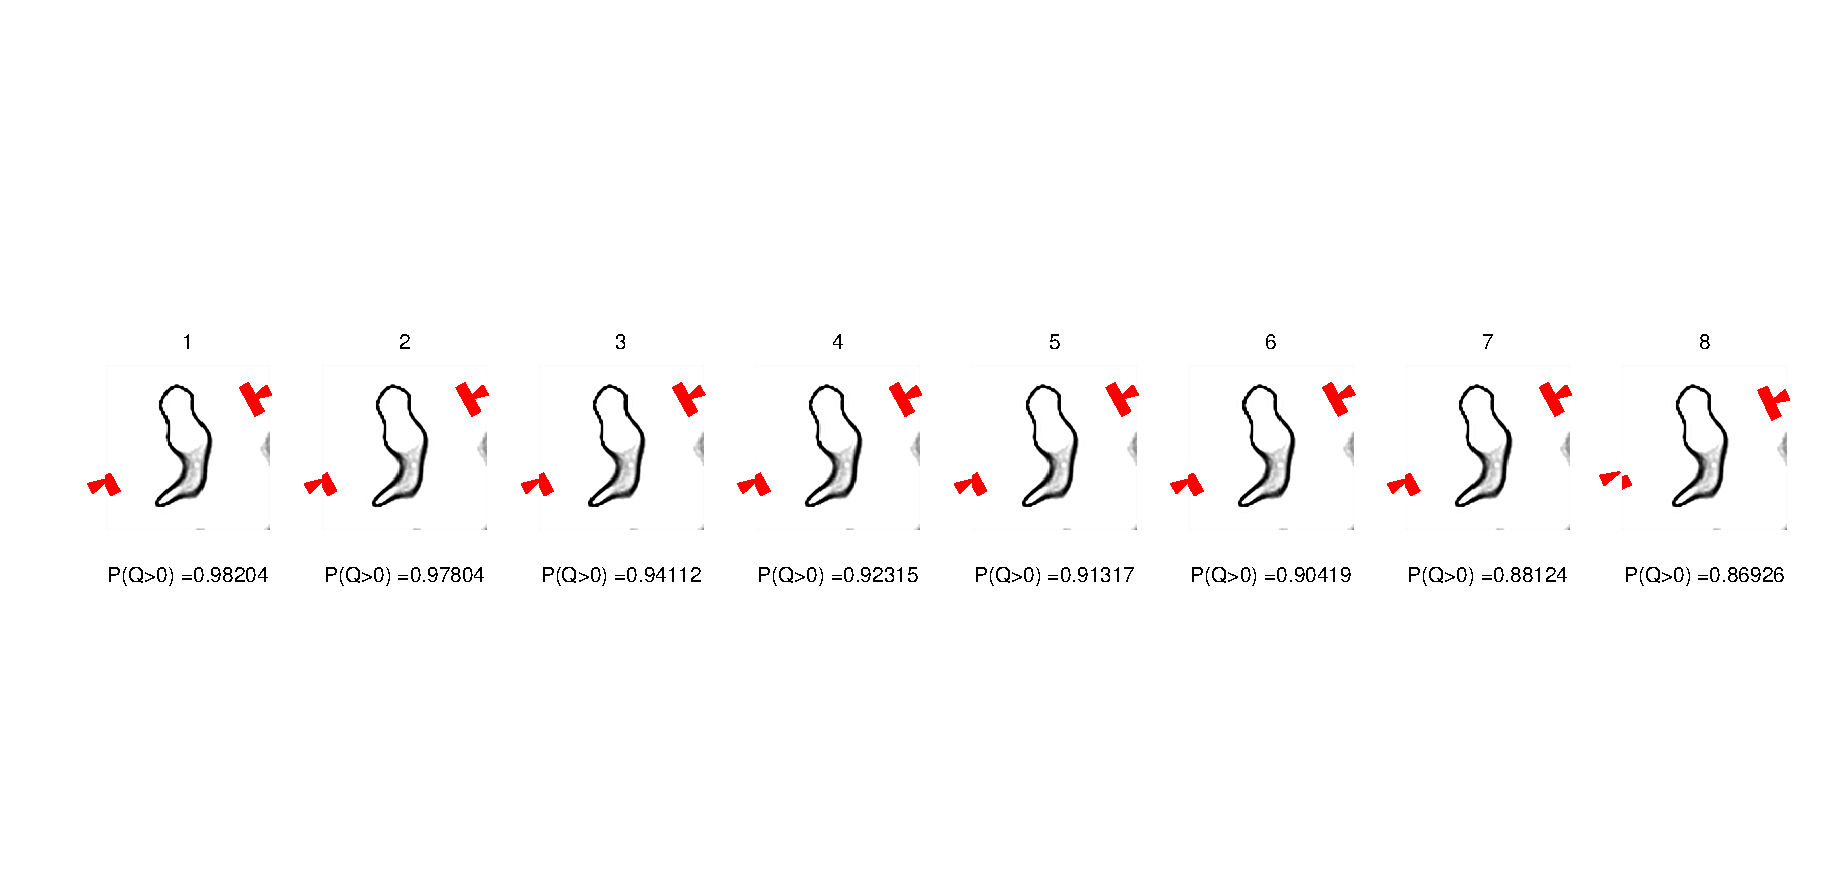
\includegraphics[width=16.5cm]{matlab_figures/rot_shapes_1.eps} }}%
    \qquad
    \subfloat[Top Grasps Shown for Shape 2]{{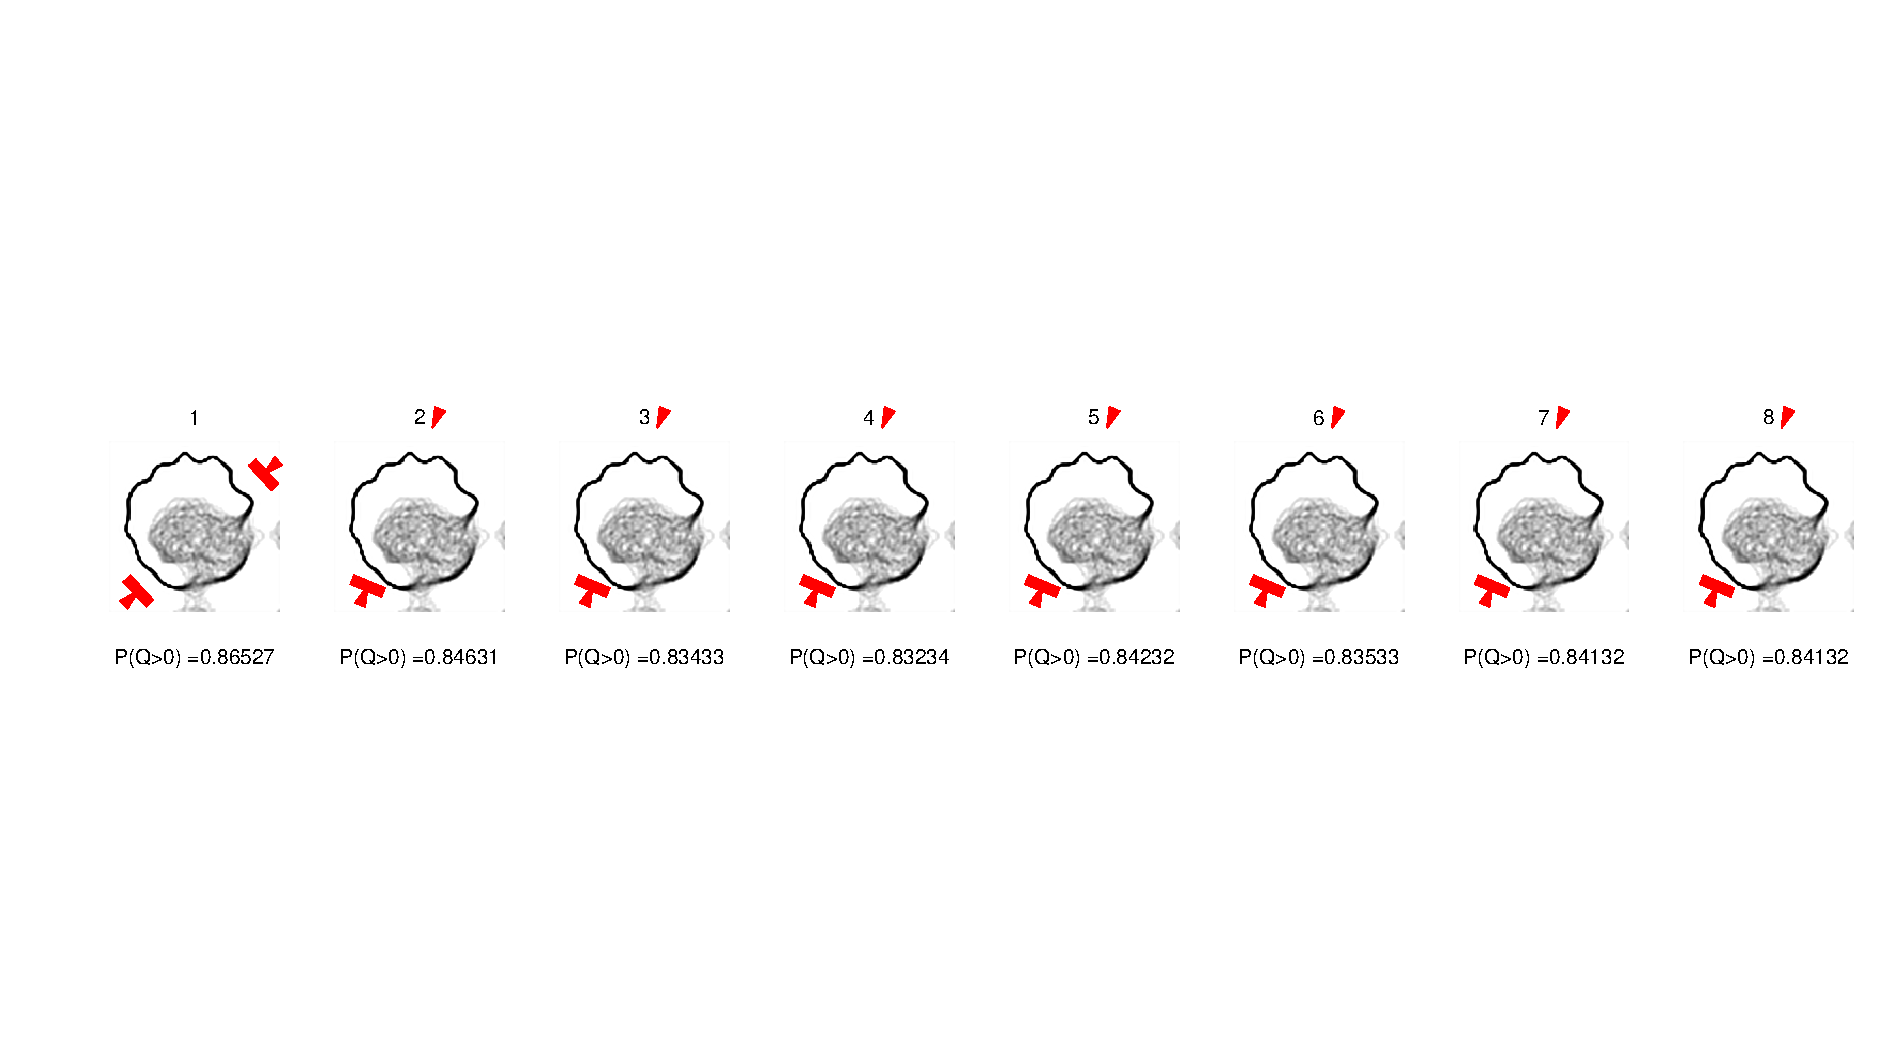
\includegraphics[width=16.5cm]{matlab_figures/rot_shapes_2.eps} }}%
    \caption{Two shapes shown from the Brown Visual Lab Dataset,from Left to Right the variance on rotation $\sigma_{rot}$ is increased $0.03$, $0.12$ to $0.24$ radians.  As you can see the overall variance increase effects the quality of the top grasp in the set of possible grasps. Furthermore for Shape 2, the grasp with low rotational variance is different than that for higher variance because the original grasp is more likely to touch the area of higher shape uncertainty when subjected to high variance in rotation. \todo{find better shapes in the brown dataset} }%
    \label{fig:rot_shapes}%
\end{figure*}


\begin{figure}[ht!]
\centering
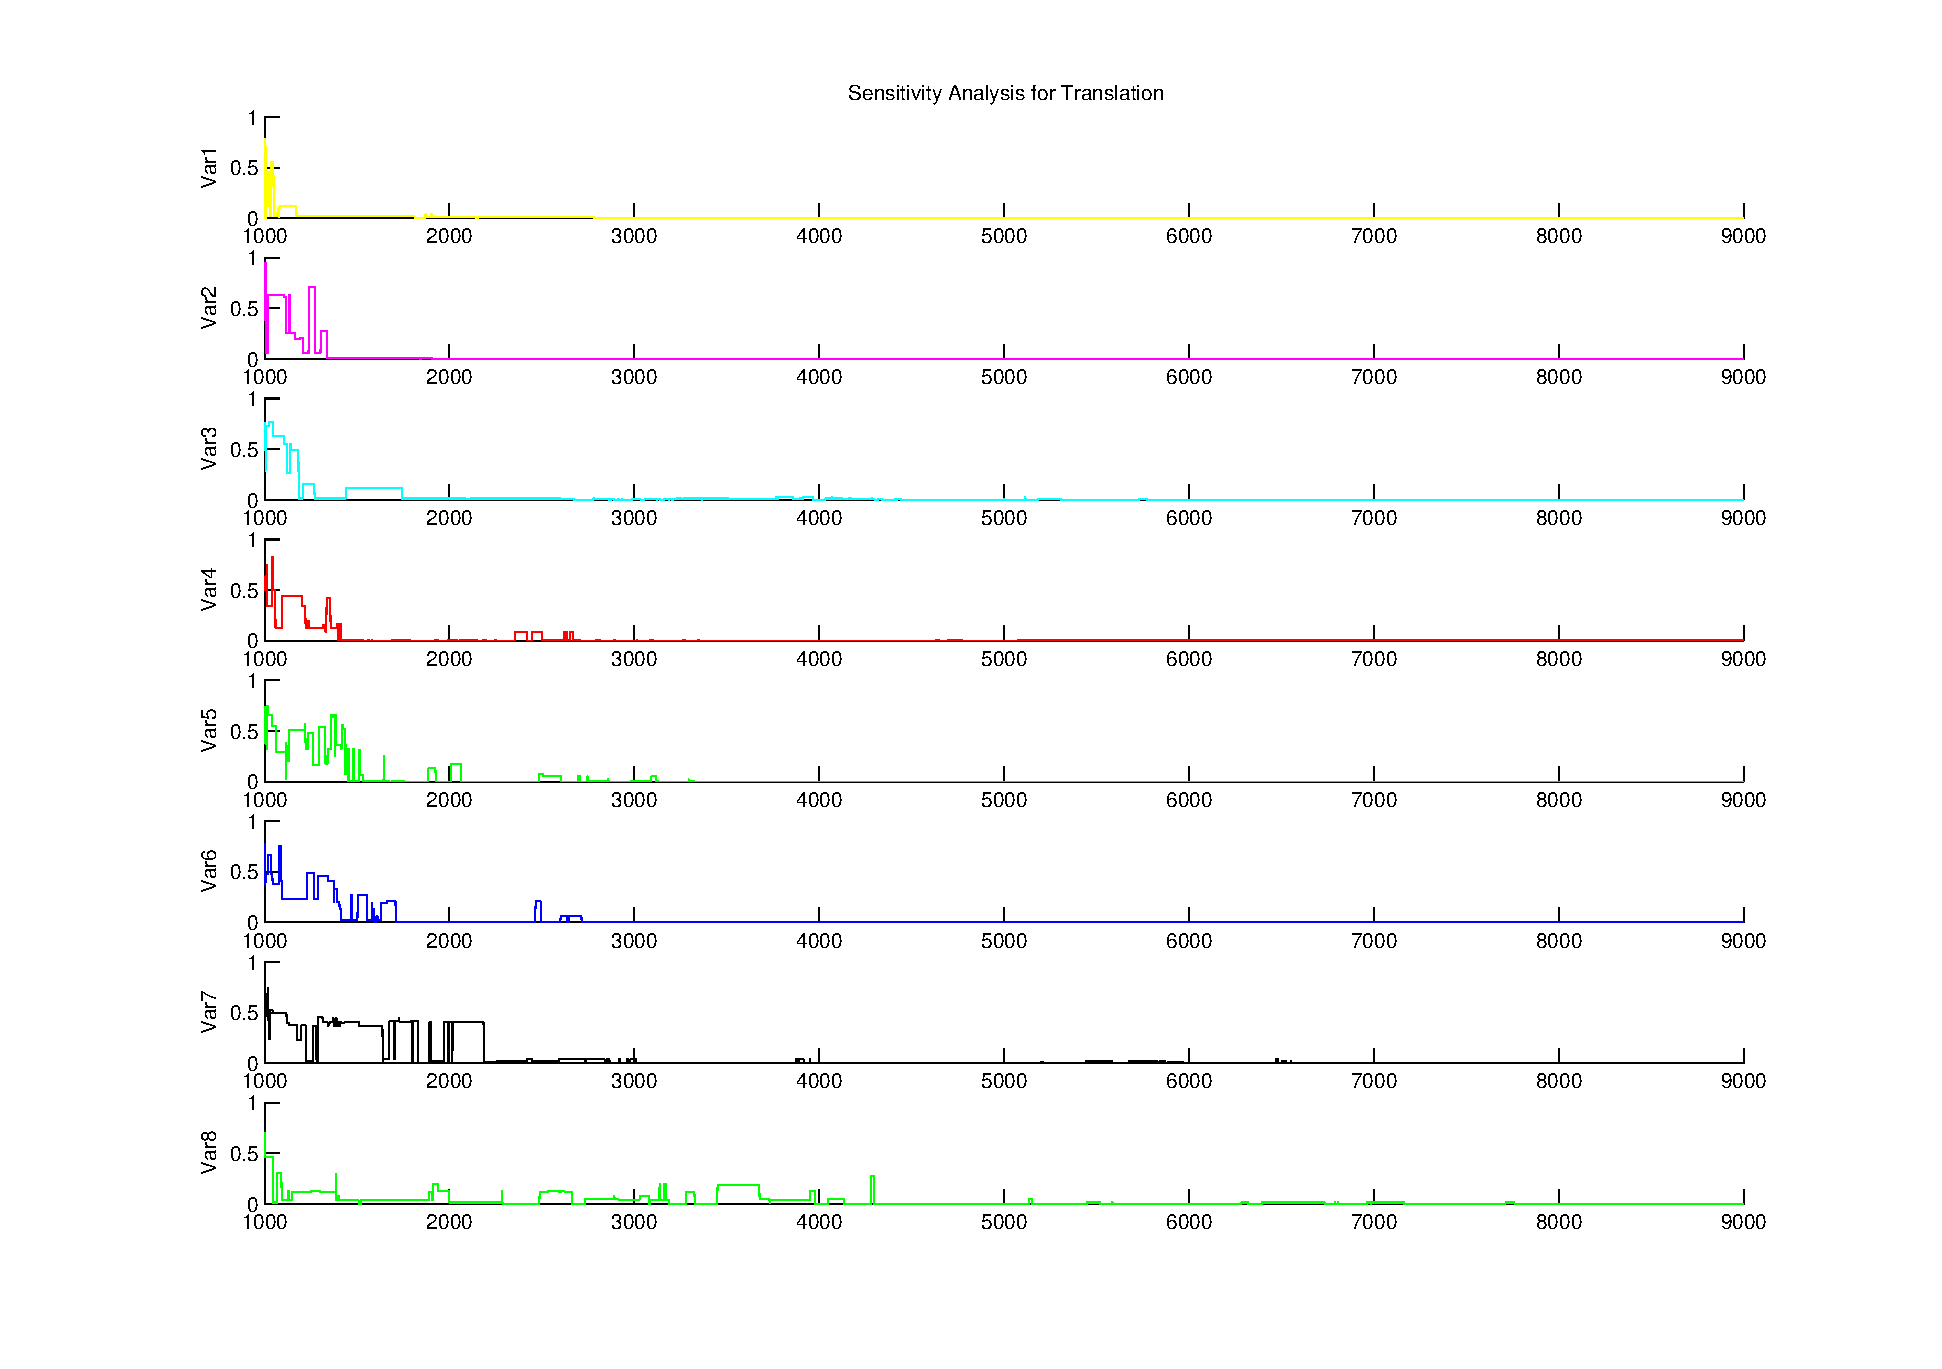
\includegraphics[width = 8cm, height = 10cm]{matlab_figures/sensitivity_trans.eps}
\caption{ \footnotesize Sensitivity Analysis for Thompson Sampling under translation uncertainty $\sigma_{trans} = \lbrace 3, 12, 24 \rbrace$ units from top to bottom on a 40 x 40 unit workspace.  As you can see the increase in noise effects performance, however the 5000 samples needed for Gittins to  converge at the the highest level of noise (which is a variance of over half the workspace) is much less that the samples needed for uniform allocation to converge in Fig. \ref{fig:simple_regret}}
\vspace*{-10pt}
\label{fig:trans_sens}
\end{figure}






\section{Limitations} 

Our budgeted multi-armed bandit approach appears promising, but we still do not know how well it will perform on 3D shapes and large scale grids. Future work will be building an efficient construction of GPIS to scale to 3D and test the bandit method there. 

The methods we showed (UCB, Thompson and Gittins) are guranteed to find the best grasp as the stopping time approaches infinity \cite{kaufmann2012bayesian,grawal2011analysis,weber1992gittins} but when do you terminate the algorithm is still an open question. Fixed confidence methods do exist that terminate when a certain confidence interval is reached \cite{maron1993hoeffding} \cite{mnih2008empirical}. However, a known problem is that if two grasps have very similar quality it could greatly increase the time for needed to reach the statistical confidence interval \cite{audibert2010best}. We proposed treating the BMAB as anytime algorithm and have demonstrated empirically that the grasps at a given stopping time are better than prior methods of Monte-Carlo sampling or the approach of Kehoe et al. However, this has a hyper parameter that has to be user-defined, which is not ideal.  

Another problem that was revealed in our analysis was that our current grasp metric, probability of force closure, is not dependent on the center of mass \cite{ferrari1992}. It only measure the probability that a grasp controller can resist any force provided it can exert an infinite force.  One can assume that the grasp controller on a robot hand is powerful enough to apply the proper resistance, but that assumption might be invalid in some applications. A similar metric that is still from Beta-Bernoulli and takes center of mass into account, would be ideal for both accurate grasp quality prediction under uncertainty and the utilization of MAB algorithms.  Recent work by Kim et al. developed a physics based simulator that could potentially achieve this goal \cite{kim2012physically}. 

\section{Conclusion}
Assessing grasp quality under  uncertainty is computationally expensive as it often requires repeated evaluations of the grasp metric over many random samples.
In this work, we proposed a multi-armed bandit approach to efficiently identify high-quality grasps under uncertainty in shape, pose, friction coeffiecient and motion. 
A key insight from our work is that uniformly allocating samples to grasps is inefficient, and
 we found that a MAB approach prioritizes evaluation of high-quality grasps while quickly pruning-out obviously poor grasps.
A pre-requisite for applying a bandit approach is to formulate a representation  of how uncertainty affects grasp parameters and thus grasp quality.
We purpose treating this as a graphical model and use model the parameters as stochastic noise. Our choice of distributions though is not the focus of the paper. The MAB algorithm is applicable in any context of bounded reward distributions and all the theoretical results we mentioned will transfer to the Beta-Bernoulli case, or the estimation of probability of force closure. 

Our anytime BMAB approach is guaranteed to find the best grasp in a given proposal set in the limit of an infinite time and has empirically been shown to outperform the methods of prior work Monte-Carlo and the method purposed by Kehoe et al. \cite{kehoe2012estimating}. 



\section{Future Work}
Our results are promising and they suggest many avenues of future work. By utilizing the BMAB model, we can encode uncertainty in the grasp parameters and then leverage the existing algorithms to efficiently find the best grasp. 

In principle, our method can be applied to other representations of shape uncertainty such as perturbations on polygonal vertices \cite{kehoe2012estimating} or splines \cite{christopoulos2007handling}.
It can further be applied to other grasp quality metrics or simulation based evaluation methods \cite{73}. 

Future work will also consider applying BMAB approach to grasp planners like GraspIt! \cite{miller2004graspit} to see if our method can handle uncertainty while working under the time constraints needed for most real time applications. While our results are promising, it remains to be seen how well it deals with the increased complexity of 3D models over 2D models and larger scale experiments. However, the BMAB model has a large amount of literature to draw from as we encounter new and more challenging problems \cite{bergemann2006bandit}.

\bibliographystyle{IEEEtranS}
\bibliography{references}


\appendix[Gaussian Process Implicit Surface for Representing Shape Uncertainty]
 \label{sec:Appendix}
 In order to solve our problem definition, we must estimate $P(Q(\Gamma)>0)$ for a given grasp . We will first discuss how the GPIS is constructed, then which grasp metric $Q$ we chose and lastly proceed into evaluating $P(Q(\Gamma)>0)$ efficiently. 


\subsection{Gaussian Process (GP) Background}\label{sec:GP}
We refer the reader to \cite{mahler2015opt} for a more detailed explanation of the GP construction, which we summarize here.  Given the training data $\mD = \{\mX, \by\}$ and covariance function $k(\cdot,\cdot)$, the posterior density $p(sd_*|\bx_*,\mD)$, or the distribution on signed distance field, at a test point $\bx_{*}$ is shown to be \cite{rasmussen2010gaussian}:
\begin{align*}
	p(sd_*|\bx_*,\mD) &\sim \mN\big(\mu(\bx_*), \Sigma(\bx_*)\big) \\
	\mu(\bx_*) &= k(\mX,\bx_*)^{\intercal}(K + \sigma^2I)^{-1}\by \\
	\Sigma(\bx_*) &= k(\bx_*,\bx_*)-k(\mX,\bx_*)^{\intercal}(K+\sigma^2I)^{-1}k(\mX,\bx_*)\big) 
\end{align*}
where $K \in \mathbb{R}^{l \times l}$ is a matrix with entries $K_{ij} = k(\bx_i,\bx_j)$ and $k(\mX,\bx_*) = [k(\bx_1,\bx_*),\ldots,k(\bx_l,\bx_*)]^{\intercal}$. 
This derivation can also be used to predict the mean and variance of the function gradient by extending the kernel matrices using the identities \cite{solak2003derivative}:

\vspace{-2ex}
\begin{align}
	\text{cov}\left(sd(\bx_i), sd(\bx_j) \right) &=  k(\bx_i, \bx_j) \\
	\text{cov}\left(\frac{\partial sd (\bx_i)}{\partial x_k}, sd(\bx_j) \right) &= \frac{\partial}{\partial x_k} k(\bx_i, \bx_j) \label{eq:mean_gradient}\\
	\text{cov}\left(\frac{\partial sd (\bx_i)}{\partial x_k}, \frac{\partial sd (\bx_j)}{\partial x_l} \right) &= \frac{\partial^2}{\partial x_k \partial x_l} k(\bx_i, \bx_j)\label{eq:cov_gradient}
\end{align}


For our kernel choice we decided to use the square exponential kernel, similar to \cite{dragiev2011}. Other kernels relevant to GPIS are the thin-plate splines kernel and the Matern kernel \cite{williams2007}. 


We construct a GPIS by learning a Gaussian process to fit measurements of a signed distance field of an unknown object.  Precisely, $x_i \in \mathbb{R}^2$ in 2D and $x_i \in \mathbb{R}^3$ in 3D, and $y_i \in \mathbb{R}$ is a noisy signed distance measurement to the unknown object at $x_i$.



\subsection{Sampling Shape from GPIS Distribution }
To compute the above distribution we must draw samples from $p(\theta)$. In order to draw shape samples from a GPIS, one needs to sample from signed distance function, $sd$, over the joint on all points in the workspace $\mathcal{W}$ or $p(sd(\mathcal{W}))$. Since this is a GPIS, we know the following 

\vspace{-2ex}
\begin{align}\label{eq:joint_shape}
p(S) = p(sd(\mathcal{W})) \sim N(\mu(\mathcal{W}),\Sigma(\mathcal{W}))
\end{align}

Thus if the workspace is an $n \times n$ grid, the joint distribution is an  $n^2$ multi-variate Gaussian, due to $sd:\mathbb{R}^2 \rightarrow \mathbb{R}$.  Shape samples drawn from the distribution appear in Fig. \ref{fig:shape_samples}.


\begin{figure}[ht!]
\centering
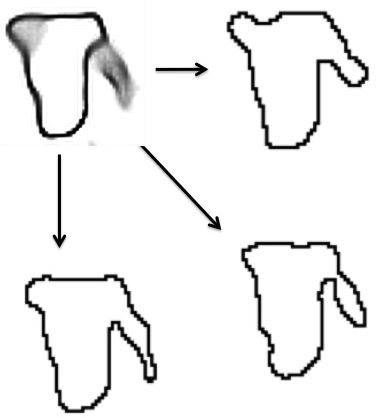
\includegraphics[width = 7.5cm, height= 6cm ]{figures/Slide13.jpg}
\caption{Shape samples drawn from Eq. \ref{eq:joint_shape} on the object in the upper left corner. Given a shape sample we highlight the zero-crossing of the level set in black}
\vspace*{-10pt}
\label{fig:shape_samples}
\end{figure}

\subsection{Distribution on Surface Normals}\label{sec:normals} 
Using Eq. \ref{eq:mean_gradient} and Eq. \ref{eq:cov_gradient}, we can compute the mean of the gradient $ \mu_{\nabla}(x)$ and the covariance of the gradient $\Sigma_{\nabla}(x)$ respectively. Thus we can compute the distribution around the surface normal for a given point in $\mathcal{W}$. We can now write 

One interesting effect of this technique is that we can now marginalize out the line of action model and visual what the surface normal distribution is along a given line of action. To our knowledge this is the first attempt to visual surface normals along a grasp plan. Marginalization can be performed as follows:

\vspace{-2ex}
\begin{equation}
    p(\textbf{n}_i ) = \int_a^b   p\big(\textbf{n}_i = \textbf{v} | \textbf{c}_i = \gamma(t) \big)p\big(\textbf{c}_i = \gamma(t)\big) dt \label{eq:normal_dist}
\end{equation}

Grasp metrics such as  Ferrari-Canny require $\textbf{n}_i$ be normalized, or, equivalently, a member of the sphere $\mathcal{S}^{d-1}$ \cite{ferrari1992}. To account for this we densely sample from the  distribution $p \big(\textbf{n}_i ) \big)$  and project onto $\mathcal{S}^{d-1}$.  In Fig.\ref{fig:GraspDist}, we visualize the distribution on $\textbf{n}_i$ calculated for a given GPIS and approach line of action.


\subsection{Expected Center of Mass}\label{sec:mass} 

We recall the quantity $P(sd(x) < 0) = \int_{-\infty}^{0} p(sd(x) =  s \ | \ \mu(x),\Sigma(x)) ds$ is equal to the probability that $x$ is interior to the surface under the current observations.
We assume that the object has uniform mass density and then $P(sd(x) < 0)$ is the expected mass density at $x$.
Then we can find the expected center of mass as:

\label{eq:mass}
\begin{equation}
  \bar{z} 
  =
  \frac
    {\int_{\mathcal{W}}x P(sd(x)<0) dx}
    {\int_{\mathcal{W}}  P(sd(x)<0) dx}
\end{equation}

which can be approximated by sampling $\mathcal{W}$ in a grid and approximating the spatial integral by a sum. Since this operation involves the entire SDF, one would want to use a low resolution grid for computational efficiency. We show the computed density and calculated expected center of mass for a marker in Fig. \ref{fig:GPIS_MASS}.


\begin{figure}[ht!]
\centering
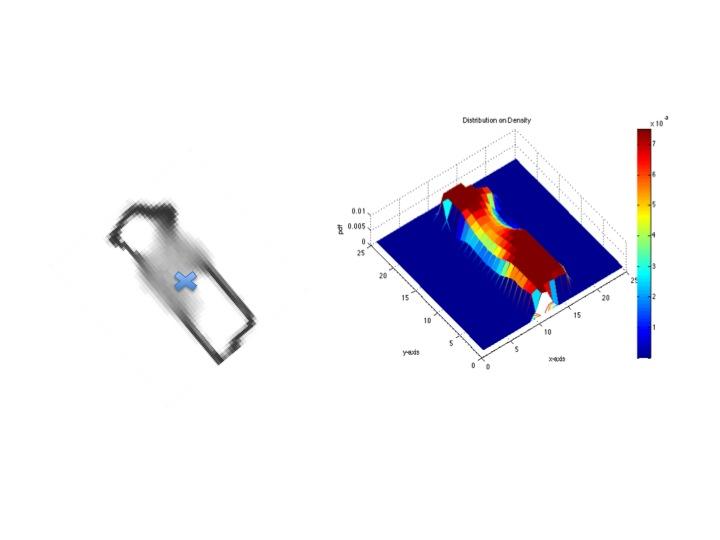
\includegraphics[scale = 0.3]{figures/Slide06.jpg}
\caption{ \footnotesize Left: A surface with GPIS construction and expected center of mass (black X)
Right: The distribution on the density of each point assuming uniform density}
\vspace*{-10pt}
\label{fig:GPIS_MASS}
\end{figure}








\end{document}
